\documentclass[a4paper, 
			   % twoside, 
			   openright, titlepage,
               headinclude, footinclude, BCOR5mm,
               numbers=noenddot, cleardoublepage=empty,
               tablecaptionabove]{scrreprt}
               
\usepackage[T1]{fontenc}
\usepackage[utf8]{inputenc}
\usepackage[english]{babel}
\usepackage{amsmath,amssymb}
\usepackage{indentfirst}
\usepackage{chngpage}
\usepackage{calc}
\usepackage{graphicx}
\usepackage{subfig}
\usepackage{lipsum}
\usepackage{shapepar}
\usepackage{pifont}
\usepackage[eulerchapternumbers,subfig,beramono,eulermath,pdfspacing,listings]{classicthesis}
\usepackage{arsclassica}
\usepackage{ccicons}

% For forcing the position of a picture
\usepackage{float}

% For wrappint the text to a picture
\usepackage{wrapfig}

% Coloring boxes in a table
\usepackage{color, colortbl}
\definecolor{LightCyan}{rgb}{0.88,1,1}

\DeclareRobustCommand*{\classicthesis}{Classic\-Thesis}
\DeclareRobustCommand*{\arsclassica}{{\normalfont\sffamily ArsClassica}}

% Necessary for correct hyperlinks (to index, bib, etc.)
\newcounter{dummy}

% Nice macros for handling all acronyms in the thesis
\usepackage{acronym}

% Code
\usepackage{listings}
\newcommand{\mail}[1]{\href{mailto:#1}{\texttt{#1}}}
\definecolor{lightergray}{gray}{0.99}
\lstset{language=python,
        keywordstyle=\color{RoyalBlue},
        basicstyle=\small\ttfamily,
        commentstyle=\color{Emerald}\ttfamily,
        stringstyle=\rmfamily,
        numberstyle=\scriptsize,
        showstringspaces=false,
        breaklines=true,
        %frame=lines, % No lines to limit the code
        backgroundcolor=\color{lightergray},
        flexiblecolumns=true,
        escapeinside={£*}{*£},
        firstnumber=last,
        numberfirstline=true,
		numbers=left,
}


% Bibliography
\usepackage[backend=biber, sorting=none]{biblatex}
\addbibresource{main.bib} % Bibliography file


\begin{document}
\pagenumbering{roman}
\pagestyle{plain}
% Titlepage

\begin{titlepage}
\pdfbookmark{Titlepage}{Titlepage}
\changetext{}{}{}{((\paperwidth  - \textwidth) / 2) - \oddsidemargin - \hoffset - 1in}{}
    \begin{center}
        {\LARGE  

        \hfill

        \vfill

        {\spacedlowsmallcaps{Omar Chehaimi}} \\ \bigskip

        {\color{Maroon}\spacedallcaps{Data Structures and Algorithms in Python}} 

        }

        \vfill

		Notes based on the Udacity online course 
		
		\today

        \vfill                      

    \end{center}        
\end{titlepage} 
\pagestyle{empty}

\hfill

\vfill


\pdfbookmark[0]{Colophon}{colophon}

\includegraphics[scale=1]{front/gfdl-logo-small.png}

This book is released into the public domain using the GNU Free Documentation License. 
	
To view a copy of the GNU Free Documentation License visit: \\\url{http://www.gnu.org/licenses/fdl-1.3.txt}
\section*{Colophon}
This document was written with \LaTeX{} using \arsclassica, a reworking of the \classicthesis{} style designed by Andr\'e Miede, inspired to the masterpiece \emph{The Elements of Typographic Style} by Robert Bringhurst.
\cleardoublepage
% Dedication

\thispagestyle{empty}
%\phantomsection 
\refstepcounter{dummy}
\pdfbookmark[1]{Dedication}{Dedication}

\vspace*{3cm}

\begin{center}
    Felix qui potuit rerum cognoscere causas.\\
	\flushright -- Publius Vergilius Maro
\end{center}
\cleardoublepage
% Preface

\chapter*{Preface}
\addcontentsline{toc}{chapter}{Preface} % Add the preface to the table of contents as a chapter

The following notes are based on the Udacity online course \href{https://www.udacity.com/course/data-structures-and-algorithms-in-python--ud513}{Intro to Data Structures and Algorithms in Python}. These notes are not intended to be a book, nor a formal introduction to data structures and algorithms, they are just my personal attempt to have a small, yet comprehensive notes about the huge world on this topic.
 
\begin{flushright}
	\textit{Omar Chehaimi}
\end{flushright}

\hfill

\vfill

\noindent
\textsf{\spacedlowsmallcaps{Contacts}}

\noindent
{\raisebox{-0.33ex}{\ding{43}}}\,\mail{omar.chehaimi@outlook.it}
\pagestyle{scrheadings} 
% Table of Contents

%\phantomsection
\refstepcounter{dummy}
\pdfbookmark[1]{\contentsname}{tableofcontents}
\setcounter{tocdepth}{2} % <-- 2 includes up to subsections in the ToC
\setcounter{secnumdepth}{3} % <-- 3 numbers up to subsubsections
\manualmark
\markboth{\spacedlowsmallcaps{\contentsname}}{\spacedlowsmallcaps{\contentsname}}
\tableofcontents 
\automark[section]{chapter}
\renewcommand{\chaptermark}[1]{\markboth{\spacedlowsmallcaps{#1}}{\spacedlowsmallcaps{#1}}}
\renewcommand{\sectionmark}[1]{\markright{\thesection\enspace\spacedlowsmallcaps{#1}}}
%*******************************************************
% List of Figures and of the Tables
%*******************************************************
\clearpage

\begingroup 
    \let\clearpage\relax
    \let\cleardoublepage\relax
    \let\cleardoublepage\relax
    %*******************************************************
    % List of Figures
    %*******************************************************    
    %\phantomsection 
    \refstepcounter{dummy}
    %\addcontentsline{toc}{chapter}{\listfigurename}
    \pdfbookmark[1]{\listfigurename}{lof}
    \listoffigures

    \vspace{8ex}

    %*******************************************************
    % List of Tables
    %*******************************************************
    %\phantomsection 
    \refstepcounter{dummy}
    %\addcontentsline{toc}{chapter}{\listtablename}
    \pdfbookmark[1]{\listtablename}{lot}
    \listoftables
        
    \vspace{8ex}
%   \newpage
    
    %*******************************************************
    % List of Listings
    %*******************************************************      
    %\phantomsection 
    \refstepcounter{dummy}
    %\addcontentsline{toc}{chapter}{\lstlistlistingname}
    \pdfbookmark[1]{\lstlistlistingname}{lol}
    \lstlistoflistings 

    \vspace{8ex}
       
    %*******************************************************
    % Acronyms
    %*******************************************************
    %\phantomsection 
    \refstepcounter{dummy}
    \pdfbookmark[1]{Acronyms}{acronyms}
    \markboth{\spacedlowsmallcaps{Acronyms}}{\spacedlowsmallcaps{Acronyms}}
    \chapter*{Acronyms}
    \begin{acronym}[UMLX]
        \acro{ADT}{Abstract data type}
        \acro{LIFO}{Last In, First Out}
        \acro{FIFO}{First In, First Out}
    \end{acronym}                     
\endgroup

\cleardoublepage
\pagenumbering{arabic}
\chapter{Preliminaries Concepts}
\label{preliminariesconcepts}

\section{Computational Complexity}
The \textbf{computational complexity}, or \textbf{complexity}, of an algorithm is the amount of resources (time and memory) needed for solving it, and it is the minimum complexity of all possible implementations for solving that given algorithm, included also the unknown ones \cite{wikipediacomplexity} (\href{https://en.wikipedia.org/wiki/Computational_complexity}{Computational complexity, Wikipedia}).

The amount of needed resources for solving an algorithm varies with the size of the input \(n\). The computational complexity in general is a function \(n \rightarrow f(n)\), and it represents the worst case complexity or the average complexity over all the inputs of size \(n\).

When the kind of the complexity is not explicitly indicated, generally is meant to be the \textbf{time complexity}, which is different from computer to computer, and it is generally expressed as the number of elementary operations required to solve a given algorithm. It is assumed that these elementary operations take the same time for being solved. The computational complexity can be related also to the memory consumption.

\section{Big O Notation}
The \textbf{big O notation} \cite{wikipediabigo} (\href{https://en.wikipedia.org/wiki/Big_O_notation}{Big O Notation, Wikipedia}) describe the behavior of a function when its argument tents to infinity or to a particular value.

\begin{definition}
Let \(f\) be a real or complex value function and let \(g\) be a real function. Let both functions be defined on the same positive and real unbounded interval, and let \(g(x)\) be strictly positive for all large enough \(x\) values: \(g(x) > 0, \forall x\) large enough. Thus: \(f(x)=O(g(x)) \) as \(x \rightarrow \infty \) if \(\exists\) \(M \in \mathbb{R} \), \(M>0\) and \(x_{0} \in \mathbb{R} \) such that \(|f(x)| \leq Mg(x)\) \(\forall x \geq x_{0}\). 
\end{definition}
Usually \(f(x)=O(g(x))\) is used as \(x \rightarrow \infty\), but it can be also defined for the case \(x \rightarrow a\), where \(a\) is a real number.

\(O\) notation is asymptotic for big \(x\), so the important terms are the ones which grow faster than the others, which become irrelevant.

\begin{example}
In \(f(x) = 6x^{4} - 2x^{3} + 5\) as \(x \rightarrow \infty\), \(6x^{4}\) it the fastest growing term. \(6\) is a constant and can be omitted, thus \(f(x)=O(x^{4})\).  
\end{example}

\subsection{Properties}
Here are listed some simple properties about Big O notation.
\begin{definition}[Product-Sum-Multiplication by a constant]
\textbf{Product} \\
\(f_{1}=O(g_{1})\) and \(f_{2}=O(g_{2})\) \(\Rightarrow\) \(f_{1}f_{2}=O(g_{1}g_{2})\)
\\
\textbf{Sum} \\
\(f_{1}=O(g_{1})\) and \(f_{2}=O(g_{2})\) \(\Rightarrow\) \(f_{1}f_{2}=O(max(f_{1}, f_{2}))\)
\\
\textbf{Multiplication by a constant} \\
Let \(k\) be a nonzero constant, then: 
\(O(k|g)=O(g)\), \(f=O(g)\) \(\Rightarrow\)\(kf=O(g)\)
\end{definition}

\begin{definition}[Logarithm and Exponential]
Let \(c\) be a nonzero constant, then: \(O(\log n^{c}) = O(\log n)\), because: (\(\log n^{c} = c \log n\)).
\\
\(O(n^{c})\) and \(O(c^{n})\) are very different, if \(c>1\) the latter grows much faster.
\\
Let \(c\) be a nonzero constant. \((cn)^{2}=c^{2}n^{2} = O(n^{2})\), but \(2^{n}\) and \(3^{n}\) are not of the same order. In general \(2^{cn}=(2^{c})^{n}\) is not of the same order of \(2^{n}\).
\end{definition}

\begin{example}
\(f = 9 \log n + 5(\log n)^{4} + 3n^{2} + 2n^{2} = O(n^{3})\) as \(n \rightarrow \infty\)
\end{example}

\begin{figure}[hb]
	\begin{center}
		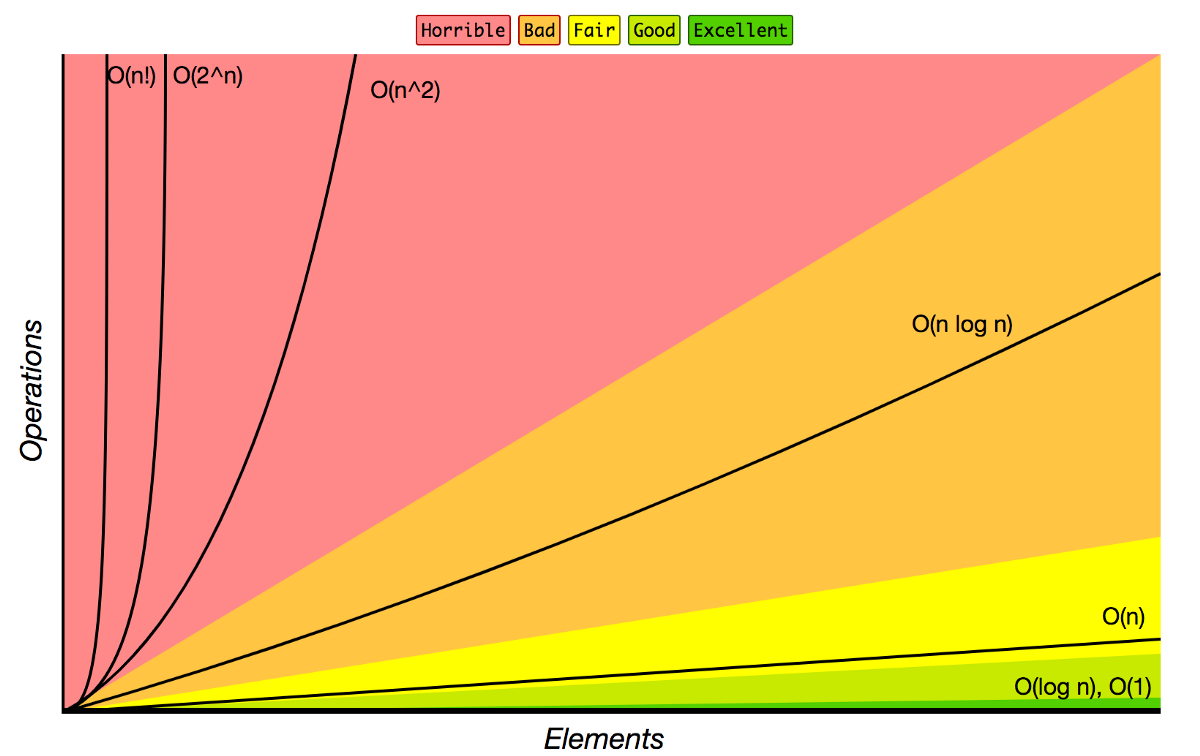
\includegraphics[scale=.3]{chapters/introduction/images/big_o_plots.png}
		\caption[Plots of the main functions and their evaluation for computational complexity.]{Plots of the main functions and their evaluation for computational complexity. Credits: \href{https://www.bigocheatsheet.com/}{bigocheatsheet.com}.}
		\label{fig:bigoplots}
	\end{center}
\end{figure}

\section{Time complexity evaluation example}
Let us suppose we want to calculate the sum of all elements of a \(n\times n\) matrix. For evaluating the time complexity of this function we have to identify all the elementary operations, and evaluating their complexity based on how many times they are repeated. Here is the pseudocode for the function that calculate the sum of a matrix.

\begin{lstlisting}[firstnumber=1, caption={Sum of all elements of a matrix.}]
def find_sum_2d(array_2d):
	totoal = 0 # -> O(1)
	for each row in array_2d: # -> repeated n times
		for each column in array_2d: # -> repeated n times
			total += array_2d[column][row] # -> O(1)
	return total # -> O(1)
\end{lstlisting}

The total time complexity is: 
\[T = O(1) + n^{2}O(1) + O(1) = O(n^{2}) \]
Where \(O(1)\) is a constant value.

\section{Recursion}
In recursion a function calls itself again on a smaller size input, until the exit condition stops this self calling (recursive calling) \cite{wikirecursion} (\href{https://en.wikipedia.org/wiki/Recursion_(computer_science)}{Recursion, Wikipedia}). There are three fundamentals elements in a recursive function:
\begin{itemize}
\item[1] A function that calls itself.
\item[2] Exit condition. Without this condition a recursive function would call itself forever without an end.
\item[3] Input alteration. When the function is called again the input is changed to a smaller dimension than the previous call.
\end{itemize}

\begin{figure}[hb]
	\begin{center}
		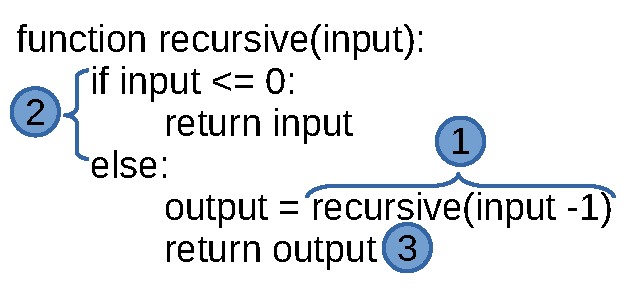
\includegraphics[scale=.6]{chapters/introduction/images/recursion_1.pdf}
		\caption[Pseudocode of a recursive function and its internal execution.]{Pseudocode of a recursive function and its internal execution.}
		\label{fig:recursion_1}
	\end{center}
\end{figure}

In recursion the exit condition is fundamental, because if it contains some errors the recursion will never end, resulting in an infinite process.

\subsection{Python Implementation Examples}

\begin{lstlisting}[firstnumber=1, caption={Implementation of the Fibonacci series with both iterative and recursive way.}]
def fibonacci_iterative(position):
	if position == 0:
		return 0
	elif position == 1:
		return 1
	else:
		first = 0
		second = 1
		next_value = first + second
		for i in range(2, position):
			first = second
			second = next
			next_value = first + second
		return next_value

def fibonacci_recursive(position):
	if position <= 1: # Exit condition
		return position
	return fibonacci(position - 1) + fibonacci(position - 2) # Calling the function on a smaller size input
\end{lstlisting}

\begin{lstlisting}[firstnumber=1, caption={Implementation of calculating the factorial of a number using the recursive way.}]
def factorial(n):
	if n <= 1: # Exit condition
		return n
	else: 
		return n*factorial(n - 1) # Calling the function on a smaller input
\end{lstlisting}

\begin{figure}[hb]
	\begin{center}
		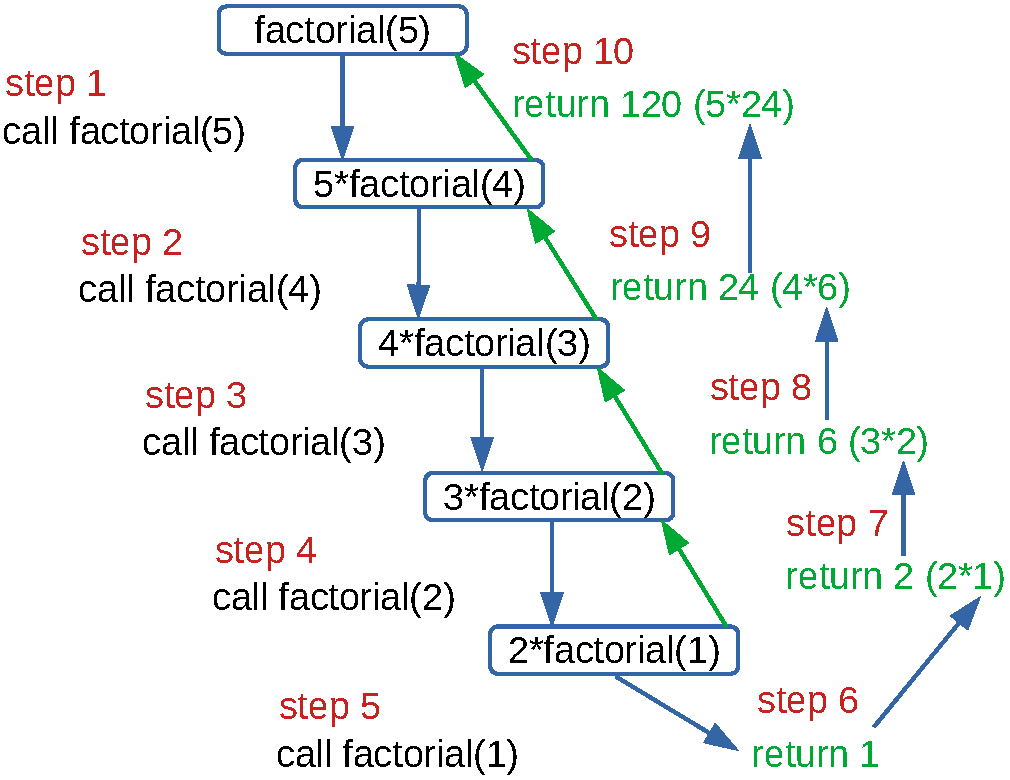
\includegraphics[scale=.6]{chapters/introduction/images/factorial.pdf}
		\caption[Factorial recursive execution.]{Factorial recursive execution.}
		\label{fig:factorial_1}
	\end{center}
\end{figure}
\chapter{Data Structures}
\label{chp:datastrucutres}
A \textbf{data structure} is a data organization, management, and storage format that enables efficient access and modification of the collected data. The relationship among collected data, their properties, the operations that can be done on them, are all properties of the data structure \cite{wikidatastructure} (\href{https://en.wikipedia.org/wiki/Data_structure}{Data Structure, Wikipedia}). Data structure is the basis for an \textbf{abstract data type (ADT)}, a mathematical model for a \textbf{data type} \cite{wikidatatype} (\href{https://en.wikipedia.org/wiki/Data_type}{Data Type, Wikipedia}), which is defined by its behavior from the point of view of a user, its type of data, specifically in terms of possible values, by possible operations on these data, and by the behavior of these operations. This mathematical model contrasts with data structures, which are concrete representations of data, and are the point of view of an implementer, not of a user \cite{wikiabstractdatatype} (\href{https://en.wikipedia.org/wiki/Abstract_data_type}{Abstract Data Type, Wikipedia}).
\\
In this chapter the most important data structures like \textbf{collections}, \textbf{lists}, \textbf{arrays}, \textbf{linked lists}, \textbf{stacks}, and \textbf{queues} are introduced. For each data structure are shown all the most important properties, operations, and implementations.
\section{Collection}
A \textbf{collection} is an object that groups several different elements in only single unit. Collections are used to save, to find, to manipulate, and to communicate grouped data \cite{wikicollection} (\href{https://en.wikipedia.org/wiki/Collection_(abstract_data_type)}{Collection (abstract data type), Wikipedia}). Usually the elements belonging to a collection are of the same type, such as a poker hand (a collection of playing cards), a folder containing emails (a collection of emails), or a phone book (a map \textit{name} \(\rightarrow\) \textit{phone number}).
\section{List}
A \textbf{list} is a collection which represents a set of \textbf{ordered} elements, which can be also of different type. Same value elements can be repeated several times. Lists do not have a fixed size, and it is possible to add, to remove, and to modify all the elements in the list. The complexity of adding or removing an element is constant (\(O(1)\)).
\section{Array}
An \textbf{array} is a collection of elements of the same or also different type, in which each of them is identified with at least one \textbf{array index} or \textbf{key} \cite{wikiarray} (\href{https://en.wikipedia.org/wiki/Array_data_structure}{Array data structure, Wikipedia}). In some programming languages arrays have a fixed size, in others instead is fixed.
\begin{figure}[H]
	\begin{center}
		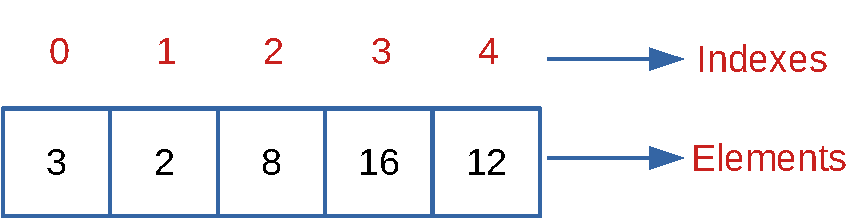
\includegraphics[scale=0.6]{chapters/datastructures/images/array_1.pdf}
		\caption[An example of an array with elements and indexes.]{An example of an array with elements and indexes.}
		\label{array_1}
	\end{center}
\end{figure}

\begin{figure}[H]
\centering
\tikzset{
mymat/.style={
  matrix of math nodes,
  text height=2.5ex,
  text depth=0.75ex,
  text width=3.25ex,
  align=center,
  column sep=-\pgflinewidth
  },
mymats/.style={
  mymat,
  nodes={draw,fill=#1}
  }  
}
\begin{tikzpicture}[node distance = 5mm and 0mm,
start chain = A going right,
box/.style = {rectangle, draw, inner sep=1mm, outer sep=0mm,
              minimum size=7mm,
                 on chain=A},
LA/.style = {-{Straight Barb[flex=0]},
               thick, shorten >=1mm, shorten <=1mm,
               looseness=1.6}, >=latex, nodes in empty cells, thick]

\matrix[mymat, anchor=east, row 2/.style={nodes=draw}]
at (0.5,0)
(mat1)
{
0 & 1 & 2 & 3 & 4 \\
8 & 2 & 4 & 1 & 7 \\
};

\draw (mat1-1-5.east)--++(0:3mm) node [right]{Indices};
\draw (mat1-2-5.east)--++(0:3mm) node [right]{Elements};

\end{tikzpicture}
\caption[An example of an array with elements and indexes.]{An example of an array with elements and indexes.}
\label{array_1}
\end{figure}

For doing any allowed operation to an element of an array it is enough to know its index. 

Adding or removing an element of an array could be a very expensive operation. This is because when a change take place to an element all the following indexes must be updated (Figure \ref{array_2}). The worst case complexity is \(O(n)\), where \(n\) is the size of the array.
\begin{figure}[H]
	\begin{center}
		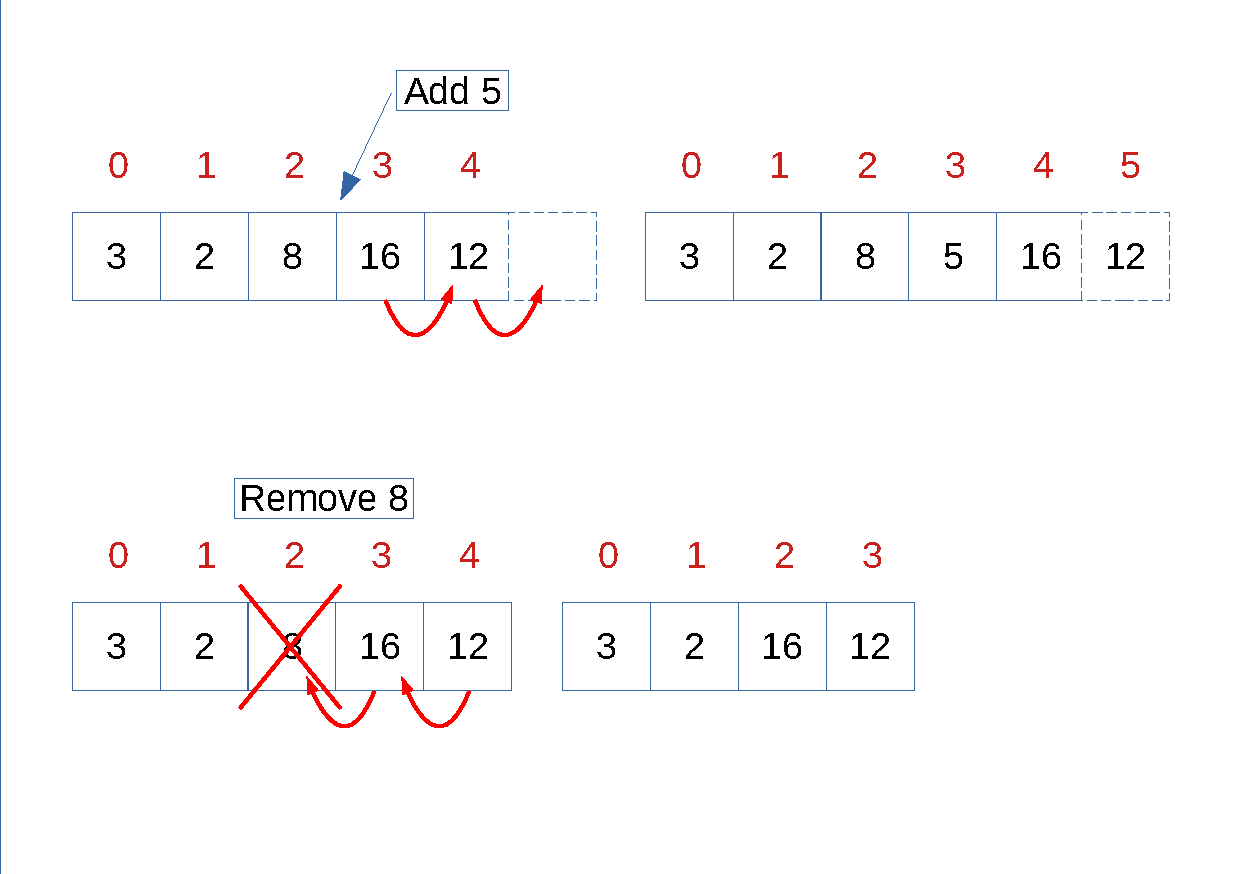
\includegraphics[scale=.6]{chapters/datastructures/images/array_2.pdf}
		\caption[Removing or adding an element from an array and the indexes update.]{Removing or adding an element from an array and the indexes update.}
		\label{array_2}
	\end{center}
\end{figure}

\begin{figure}[H]
\centering
\tikzset{
mymat/.style={
  matrix of math nodes,
  text height=2.5ex,
  text depth=0.75ex,
  text width=3.25ex,
  align=center,
  column sep=-\pgflinewidth
  },
mymats/.style={
  mymat,
  nodes={draw,fill=#1}
  }  
}
\begin{subfigure}[b]{\linewidth}
\centering
\begin{tikzpicture}[node distance = 5mm and 0mm,
start chain = A going right,
box/.style = {rectangle, draw, inner sep=1mm, outer sep=0mm,
              minimum size=7mm,
                 on chain=A},
LA/.style = {-{Straight Barb[flex=0]},
               thick, shorten >=1mm, shorten <=1mm,
               looseness=1.6}, >=latex, nodes in empty cells, thick]

\matrix[mymat, anchor=east, row 2/.style={nodes=draw}, 
        column 5/.style={nodes=densely dashed}]
at (0.5,0)
(mat1)
{
0 & 1 & 2 & 3 & \\
8 & 2 & 4 & 1 & \\
};
\matrix[mymat, anchor=west, row 2/.style={nodes=draw}, column 5/.style={nodes=densely dashed}] at (0.5,0)
(mat2)
{
0 & 1 & 2 & 3 & 4 \\
8 & 2 & 9 & 4 & 1 \\
};

\draw ($(mat1-2-3.north) + (-1mm, 10mm)$) node[draw=none, rectangle, align=left] (r1) {add 9};

\draw[->, >=stealth, BrickRed] (r1.south) -- (mat1-2-2.north east);

\path[->, >=stealth, BrickRed] (mat1-2-3.south) edge [bend right=60] node[draw=none] {} (mat1-2-4.south);
\path[->, >=stealth, BrickRed] (mat1-2-4.south) edge [bend right=60] node[draw=none] {} (mat1-2-5.south);

\end{tikzpicture}
\caption{Adding an element to an array.}
\label{adding_arr}
\end{subfigure}
%\hspace{1em}
\begin{subfigure}[b]{\linewidth}
\centering
\begin{tikzpicture}[node distance = 5mm and 0mm,
start chain = A going right,
box/.style = {rectangle, draw, inner sep=1mm, outer sep=0mm,
              minimum size=7mm,
                 on chain=A},
LA/.style = {-{Straight Barb[flex=0]},
               thick, shorten >=1mm, shorten <=1mm,
               looseness=1.6}, >=latex, nodes in empty cells, thick]

\matrix[mymat, anchor=east, row 2/.style={nodes=draw}] at (-1.4,0) (mat1)
{
0 & 1 & 2 & 3 \\
8 & 2 & 4 & 1 \\
};
\matrix[mymat, anchor=west, row 2/.style={nodes=draw}] at (-1.4,0)
(mat2)
{
0 & 1 & 2 \\
8 & 4 & 1 \\
};

\draw[BrickRed, style={-}] ($(mat1-2-2) + (-0.5,0.5)$) -- ($(mat1-2-2) + (0.5,-0.5)$);
\draw[BrickRed, style={-}] ($(mat1-2-2) + (0.5,0.5)$) -- ($(mat1-2-2) + (-0.5,-0.5)$);

\path[->, >=stealth, BrickRed] (mat1-2-4.south) edge [bend left=60] node[draw=none] {} (mat1-2-3.south);
\path[->, >=stealth, BrickRed] (mat1-2-3.south) edge [bend left=60] node[draw=none] {} (mat1-2-2.south);

\end{tikzpicture}
\caption{Removing an element to an array.}
\label{removing_arr}
\end{subfigure}
\caption[Adding \ref{adding_arr} or removing \ref{removing_arr} an element from an array and the indexes update.]{Adding \ref{adding_arr} or removing \ref{removing_arr} an element from an array and the indexes update.}
\label{array_2}
\end{figure}

\section{Linked List}
\label{linkedlist}
A \textbf{linked list} is a linear collection in which each element has the data and a reference to the next element (a link) \cite{wikilinkedlist} (\href{https://en.wikipedia.org/wiki/Linked_list}{Linked List, Wikipedia}). 
\begin{figure}[H]
	\begin{center}
		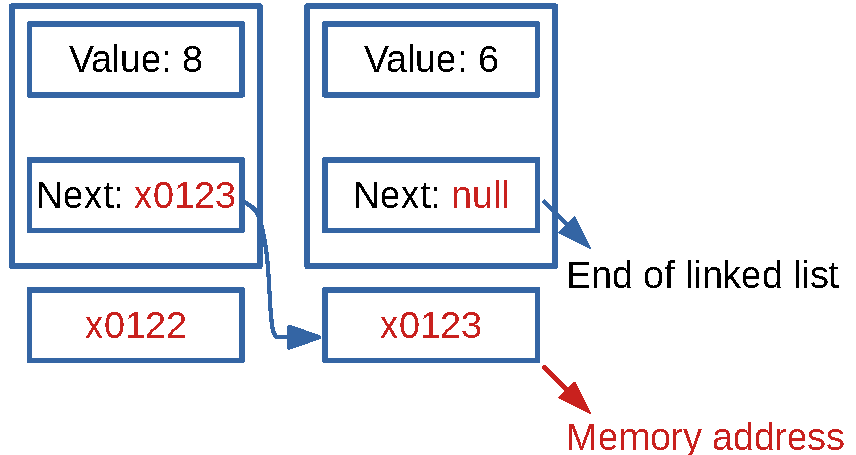
\includegraphics[scale=.6]{chapters/datastructures/images/linked_list_1.pdf}
		\caption[An example of a linked list with the data and the reference to the next element.]{An example of a linked list with the data and the reference to the next element.}
		\label{linked_list_1}
	\end{center}
\end{figure}

\begin{figure}[H]
\centering
\begin{tikzpicture}[double link/.style n args=2{on chain, rectangle split, rectangle split horizontal, rectangle split parts=2, draw, anchor=center, text height=1.5ex, node contents={#1\nodepart{two}#2},}, start chain=going right, >=stealth, thick, node distance=15mm]

\node[double link={$Head$}{\textcolor{BrickRed}{$0x00$}}, alias={h}];
\node[join={by ->}, double link={$7$}{\textcolor{BrickRed}{$0x01$}}, alias={a}];
\node[join={by ->}, double link={$1$}{\textcolor{BrickRed}{$0x02$}}, alias={b}];
\node[join={by ->}, double link={$13$}{\textcolor{BrickRed}{$null$}}, alias={c}];

\draw ($(a) + (0,-5mm)$) node[draw=none, rectangle, align=left] (r1) {\textcolor{BrickRed}{$0x00$}};
\draw ($(b) + (0,-5mm)$) node[draw=none, rectangle, align=left] (r2) {\textcolor{BrickRed}{$0x01$}};
\draw ($(c) + (0,-5mm)$) node[draw=none, rectangle, align=left] (r3) {\textcolor{BrickRed}{$0x02$}};

\draw ($(a) + (0,1)$) node[draw=none, rectangle, align=left] (r3) {Content};
\draw ($(a) + (4,1)$) node[draw=none, rectangle, align=left] (r4) {Address (pointer) of the next node};
\draw ($(c) + (2.4,0)$) node[draw=none, rectangle, align=left] (r5) {Last node \\ points to null};

\draw[->, >=stealth] (r3.south) -- (a.one north);
\draw[->, >=stealth] (r4.south) -- (a.two north);
\draw[->, >=stealth] (r5.west) -- (c.two east); 
\end{tikzpicture}

\caption[An example of a linked list with the data and the reference to the next element.]{An example of a linked list with the data and the reference to the next element.}
\label{linked_list_1}
\end{figure}

In a linked list the order of the elements is not assured. 

Operations like adding or removing an element in a linked list are very efficient, because it is enough to change the references of the elements involved in the operation. For example for adding a new element is enough to change the previous element reference to the just added element, and change the reference of the new element to the next element (Figure \ref{linked_list_2}). In case of removing an element it is enough to update the previous element's reference to the next element of the removed one (Figure \ref{linked_list_3}). 
\begin{figure}[H]
	\begin{center}
		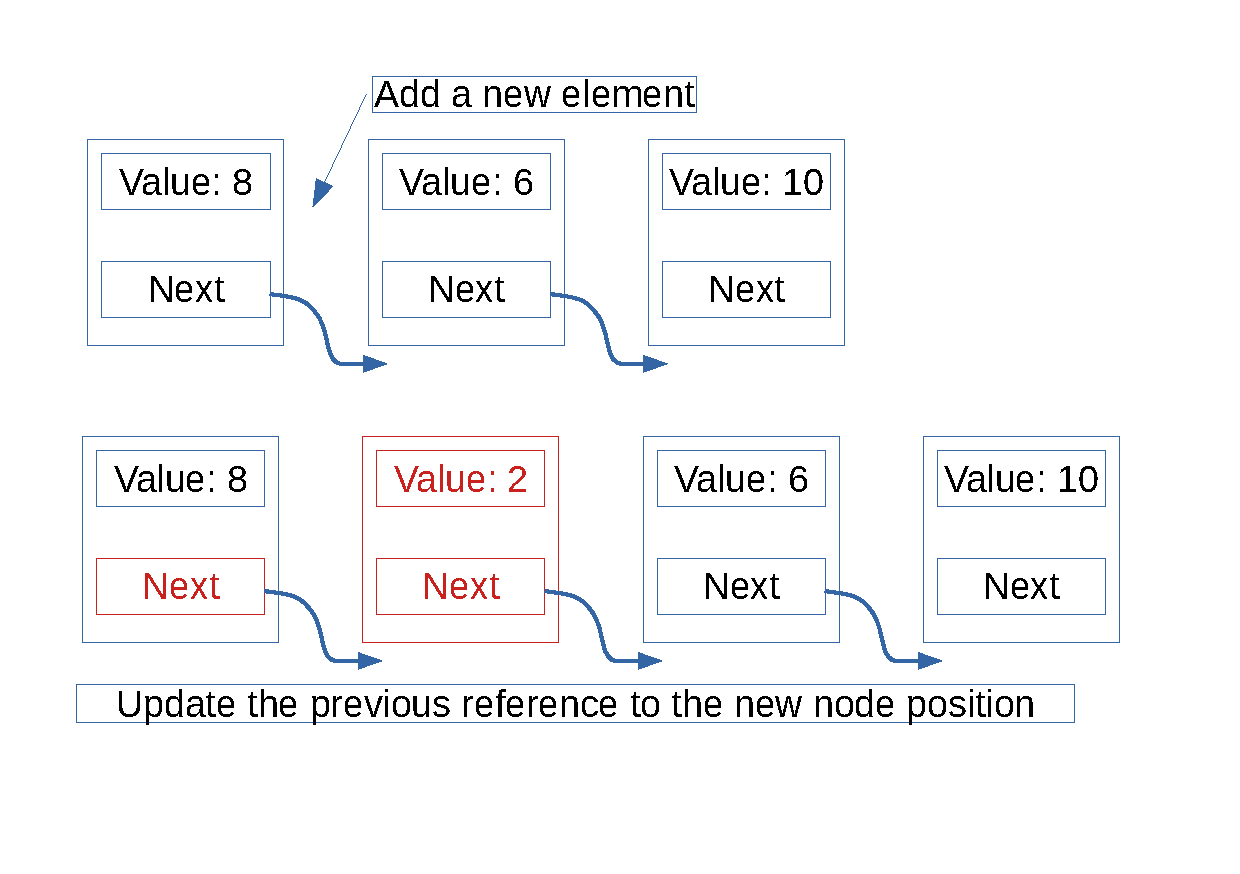
\includegraphics[scale=.6]{chapters/datastructures/images/linked_list_2.pdf}
		\caption[Adding a new element to a linked list.]{Adding a new element to the linked list. As explained before this operation is very efficient because it is enough to change the references of the new element and the previous element to the one just added.}
		\label{linked_list_2}
	\end{center}
\end{figure}

\begin{figure}[H]
\centering
\begin{tikzpicture}[double link/.style n args=2{on chain, rectangle split, rectangle split horizontal, rectangle split parts=2, draw, anchor=center, text height=1.5ex, node contents={#1\nodepart{two}#2},}, start chain=going right, >=stealth, thick, node distance=15mm]

\node[double link={$Head$}{\textcolor{BrickRed}{$0x00$}}, alias={h}];
\node[join={by ->}, double link={$7$}{\textcolor{BrickRed}{$0x01$}}, alias={a}];
\node[join={by ->}, double link={$1$}{\textcolor{BrickRed}{$0x02$}}, alias={b}];
\node[join={by ->}, double link={$13$}{\textcolor{BrickRed}{$null$}}, alias={c}];

\draw ($(a) + (0,-5mm)$) node[draw=none, rectangle, align=left] (r1) {\textcolor{BrickRed}{$0x00$}};
\draw ($(b) + (0,-5mm)$) node[draw=none, rectangle, align=left] (r2) {\textcolor{BrickRed}{$0x01$}};
\draw ($(c) + (0,-5mm)$) node[draw=none, rectangle, align=left] (r3) {\textcolor{BrickRed}{$0x02$}};
\draw ($(a) + (-5mm,10mm)$) node[draw=none, rectangle, align=left] (r4) {Add a new element};
\draw[->, >=stealth] (r4.south) -- (1.5,0);
\end{tikzpicture}

\begin{tikzpicture}[double link/.style n args=2{on chain, rectangle split, rectangle split horizontal, rectangle split parts=2, draw, anchor=center, text height=1.5ex, node contents={#1\nodepart{two}#2},}, start chain=going right, >=stealth, thick, node distance=15mm]

\node[double link={$Head$}{\textcolor{BrickRed}{$0x04$}}, alias={h}];
\node[join={by ->}, double link={$3$}{\textcolor{BrickRed}{$0x00$}}, alias={aa}, BrickRed];
\node[join={by ->}, double link={$7$}{\textcolor{BrickRed}{$0x01$}}, alias={a}];
\node[join={by ->}, double link={$1$}{\textcolor{BrickRed}{$0x02$}}, alias={b}];
\node[join={by ->}, double link={$13$}{\textcolor{BrickRed}{$null$}}, alias={c}];

\draw ($(aa) + (0,-5mm)$) node[draw=none, rectangle, align=left] (r11) {\textcolor{BrickRed}{$0x04$}};
\draw ($(a) + (0,-5mm)$) node[draw=none, rectangle, align=left] (r1) {\textcolor{BrickRed}{$0x00$}};
\draw ($(b) + (0,-5mm)$) node[draw=none, rectangle, align=left] (r2) {\textcolor{BrickRed}{$0x01$}};
\draw ($(c) + (0,-5mm)$) node[draw=none, rectangle, align=left] (r3) {\textcolor{BrickRed}{$0x02$}};
\end{tikzpicture}

\caption[Adding a new element to a linked list.]{Adding a new element to the linked list. As explained before this operation is very efficient because it is enough to change the references of the new element and the previous element to the one just added.}
\label{linked_list_2}
\end{figure}

\begin{figure}[H]
	\begin{center}
		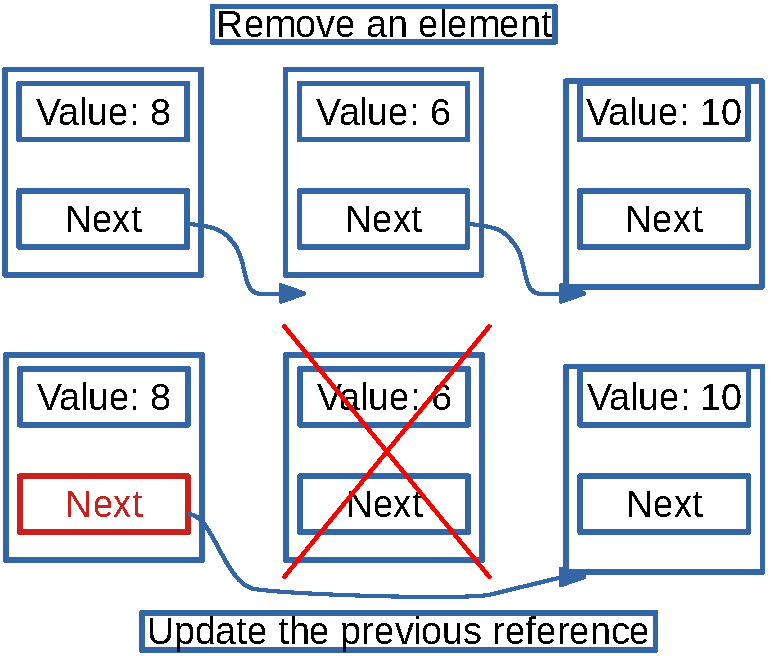
\includegraphics[scale=.6]{chapters/datastructures/images/linked_list_3.pdf}
		\caption[Removing an element to a linked list.]{Removing an element to a linked list.}
		\label{linked_list_3}
	\end{center}
\end{figure}

\begin{figure}[H]
\centering
\begin{tikzpicture}[double link/.style n args=2{on chain, rectangle split, rectangle split horizontal, rectangle split parts=2, draw, anchor=center, text height=1.5ex, node contents={#1\nodepart{two}#2},}, start chain=going right, >=stealth, thick, node distance=15mm]

\node[double link={$Head$}{\textcolor{BrickRed}{$0x00$}}, alias={h}];
\node[join={by ->}, double link={$7$}{\textcolor{BrickRed}{$0x01$}}, alias={a}];
\node[join={by ->}, double link={$1$}{\textcolor{BrickRed}{$0x02$}}, alias={b}];
\node[join={by ->}, double link={$13$}{\textcolor{BrickRed}{$null$}}, alias={c}];

\draw ($(a) + (0,-5mm)$) node[draw=none, rectangle, align=left] (r1) {\textcolor{BrickRed}{$0x00$}};
\draw ($(b) + (0,-5mm)$) node[draw=none, rectangle, align=left] (r2) {\textcolor{BrickRed}{$0x01$}};
\draw ($(c) + (0,-5mm)$) node[draw=none, rectangle, align=left] (r3) {\textcolor{BrickRed}{$0x02$}};

\draw[BrickRed, style={-}] ($(a) + (-0.5,0.5)$) -- ($(a) + (0.5,-0.5)$);
\draw[BrickRed, style={-}] ($(a) + (0.5,0.5)$) -- ($(a) + (-0.5,-0.5)$);
\end{tikzpicture}

\begin{tikzpicture}[double link/.style n args=2{on chain, rectangle split, rectangle split horizontal, rectangle split parts=2, draw, anchor=center, text height=1.5ex, node contents={#1\nodepart{two}#2},}, start chain=going right, >=stealth, thick, node distance=15mm]

\node[double link={$Head$}{\textcolor{BrickRed}{$0x01$}}, alias={h}];
\node[join={by ->}, double link={$1$}{\textcolor{BrickRed}{$0x02$}}, alias={b}];
\node[join={by ->}, double link={$13$}{\textcolor{BrickRed}{$null$}}, alias={c}];

\draw ($(b) + (0,-5mm)$) node[draw=none, rectangle, align=left] (r2) {\textcolor{BrickRed}{$0x01$}};
\draw ($(c) + (0,-5mm)$) node[draw=none, rectangle, align=left] (r3) {\textcolor{BrickRed}{$0x02$}};
\end{tikzpicture}

\caption[Removing an element to a linked list.]{Removing an element to a linked list.}
\label{linked_list_3}
\end{figure}

The complexity for adding or removing an element is constant \(O(1)\).
Linked lists can be also \textbf{doubly linked list} (Figure \ref{linked_list_4}), which evry element has the reference to the previous and next element of the collection \cite{wikidoublylinkedlist} (\href{https://en.wikipedia.org/wiki/Doubly_linked_list}{Doubly linked list, Wikipedia}).
\begin{figure}[H]
	\begin{center}
		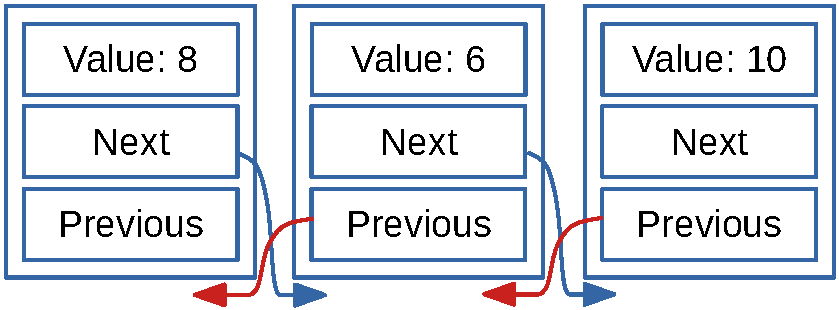
\includegraphics[scale=.6]{chapters/datastructures/images/linked_list_4.pdf}
		\caption[Doubly linked list.]{Doubly linked list.}
		\label{linked_list_4}
	\end{center}
\end{figure}

\begin{figure}[H]
\centering
\begin{tikzpicture}[list/.style={thick, rectangle split, rectangle split parts=3, draw, rectangle split horizontal, minimum size=18pt, inner sep=5pt, text=black}, ->, start chain, thick]

  \node[list, on chain] (a) {\nodepart{second} $7$};
  \node[list, on chain] (b) {\nodepart{second} $1$};
  \node[list, on chain] (c) {\nodepart{second} $13$};

  \node[draw, rectangle, minimum size=18pt] (d) [right=of c] {\textcolor{BrickRed}{$null$}};
  \node[draw, rectangle, minimum size=18pt] (e) [left= of a] {\textcolor{BrickRed}{$null$}};
  
  \draw[*->, >=stealth] ($(a.one) + (0.2, 0.1)$) -- (e.east);
   
  \path[*->] let \p1 = (a.three), \p2 = (a.center) in (\x1,\y2) edge [bend left] ($(b.one)+(0,0.2)$);
  \path[*->] ($(b.one)+(0.1,0.1)$) edge [bend left] ($(a.three)+(0,-0.05)$);
  \path[*->] let \p1 = (b.three), \p2 = (b.center) in (\x1,\y2) edge [bend left] ($(c.one)+(0,0.2)$);
  
  \draw[*->] let \p1 = (c.three), \p2 = (c.center) in (\x1,\y2) -- (d);
  \path[*->] ($(c.one)+(0.1,0.1)$) edge [bend left] ($(b.three)+(0,-0.05)$);
\end{tikzpicture}
\caption[Doubly linked list.]{Doubly linked list.}
\label{linked_list_4}
\end{figure}

Linked list are used for implementing other data structures such as lists, stacks, queues, and associative array.

\subsection{Linked List Implementation}
The following code is the implementation of a linked list in Python.
\begin{lstlisting}[firstnumber=1, caption={Linked List implementation.}]
class Element():

	def __init__(self, value):
		self.value = value
		self.next = None
		
class LinkedList():

	def __init__(self, head=None):
		self.head = head
		
	def append(self, new_element):
		current = self.head
		if self.head:
			while current.next:
				current = current.next
			current.next = new_element
		else:
			self.head = new_element
	
	def get_position(self, position):
		counter = 0
		current = self.head
		if position < 1:
			return None
		while current and counter <= position:
			if counter == position:
				return current
			current = current.next
			counter += 1
		return None
	
	def insert(self, new_element, position):
		counter = 1
		current = self.head
		if position > 1:
			while current and counter < position:
				if counter == position - 1:
					new_element.next = current.next
					current.next = new_element
				current = current.next
				counter +=1 
		elif position == 1:
			new_element.next = self.head
			self.head = new_element
\end{lstlisting}

\section{Stack}
\label{stack}
A \textbf{stack} is abstract data type belonging to collections, in which only two operations are allowed \cite{wikistack} (\href{https://en.wikipedia.org/wiki/Stack_(abstract_data_type)}{Stack, Wikipedia}):
\begin{itemize}
\item[•] \textbf{Push}: add an element at the top of the stack
\item[•] \textbf{Pop}: remove the newest element of the stack
\end{itemize}
In the stacks only the element at the top of the stack can be modified. The complexity remains constant for adding and removing operations. The stacks are also called \textbf{Last In, First Out} (\textbf{LIFO}).
\begin{figure}[H]
	\begin{center}
		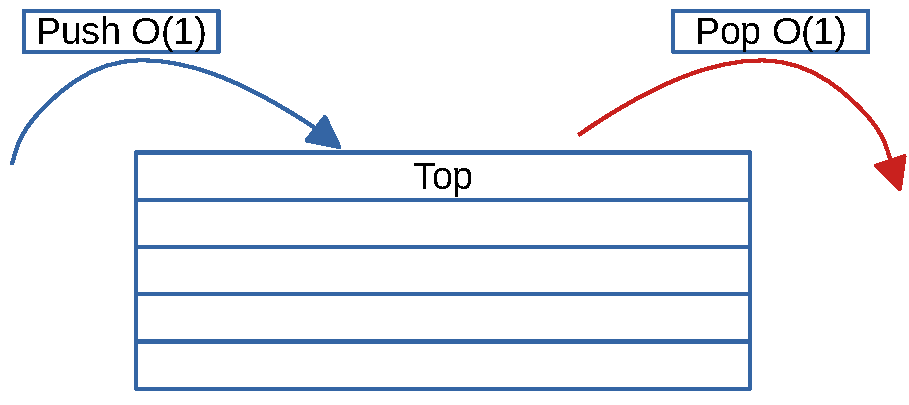
\includegraphics[scale=.6]{chapters/datastructures/images/stack_1.pdf}
		\caption[In a stack only the element at the top is modified.]{In a stack only the element at the top is modified.}
		\label{stack_1}
	\end{center}
\end{figure}

\begin{figure}[H]
\centering
\begin{tikzpicture}[draw, minimum width=1.5cm, minimum height=0.5cm, thick]
    \node[draw] (push) at (-1,2) {};
    \node[draw=none] at ($(push) + (0, 5mm)$) {Push $O(1)$};
    \node[draw] (pop) at (1,2) {};
    \node[draw=none] at ($(pop) + (0, 5mm)$) {Pop $O(1)$};
    
    \matrix (queue)[matrix of nodes, nodes={draw, nodes={draw}}, nodes in empty cells, row sep=-\pgflinewidth]
    {
       \\ \\ \\ \\
    };

    \draw[->, >=stealth] (0.25,1) -- (pop.south);
    \draw[->, >=stealth] (push.south) -- (-0.25,1);
\end{tikzpicture}
\caption[In a stack only the element at the top is modified.]{In a stack only the element at the top is modified.}
\label{stack_1}
\end{figure}

\subsection{Stack Implementation}
The following is the implementation in Python of a stack using the linked list.
\begin{lstlisting}[firstnumber=1, caption={Stack implementation.}]
class Element():
	...

class LinkedList():
	...
	
	def insert_first(self, new_element):
		new_element.next = self.head
		self.head = new_element
	
	def delete_first(self):
		if self.head:
			delete_element = self.head
			temp = deleted_element.next
			self.head = temp
			return deleted_element
		else:
			return None

class Stack():
	
	def __init__(self, top=None):
		self.ll = LinkedList(top)
		
	def push(self, new_element):
		self.ll.insert_first(new_element)
	
	def pop(self):
		self.ll.delete_first()
\end{lstlisting}

\section{Queue}
\label{queue}
A \textbf{queue} is abstract data type belonging to collections very similar to the stacks. For a queue the admitted operations are only on the oldest element, thus the first element to be added \cite{wikiqueue} (\href{https://en.wikipedia.org/wiki/Queue_(abstract_data_type)}{Queue, Wikipedia}). The allowed operations on a queue are:
\begin{itemize}
\item[•] \textbf{Enque}: adding an element at the bottom of the queue
\item[•] \textbf{Deque}: removing the element at the head of the queue
\item[•] \textbf{Pick}: observing the element at the head of the queue
\end{itemize}
For adding and removing operations the complexity remain constant. Queues are also called \textbf{First In, First Out} (\textbf{FIFO}). 

The most efficient way to implement a queue is using linked lists.

\begin{figure}[H]
	\begin{center}
		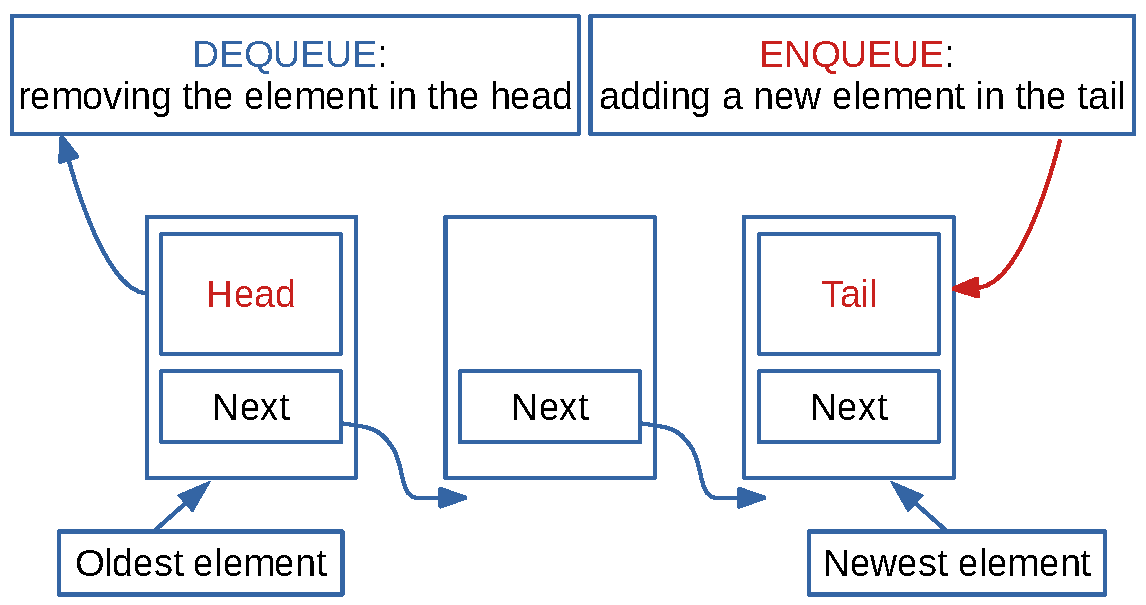
\includegraphics[scale=.6]{chapters/datastructures/images/queue_1.pdf}
		\caption[Allowed operations on queue elements.]{In a queue only the first element to be added can be removed or where a new element can be added.}
		\label{queue_1}
	\end{center}
\end{figure}

\begin{figure}[H]
\centering
\begin{tikzpicture}[draw, minimum width=1.5cm, minimum height=0.5cm, thick]  
    \node[draw] (enqueue) at (-1,2) {};
    \node[draw=none] at ($(enqueue) + (0, 5mm)$) {Enqueue $O(1)$};
    \node[draw] (dequeue) at (1,-2) {};
    \node[draw=none] at ($(dequeue) + (0, -5mm)$) {Dequeue $O(1)$};
    
    \matrix (queue)[matrix of nodes, nodes={draw, nodes={draw}}, nodes in empty cells, row sep=-\pgflinewidth]
    {
      Head \\ 
       \\ 
       \\ 
       Tail \\
    };

    \draw[->, >=stealth] (0.25,-1.05) -- (dequeue.north);
    \draw[->, >=stealth] (enqueue.south) -- (-0.25,1.05);
\end{tikzpicture}
\caption[Allowed operations on queue elements.]{In a queue only the first element to be added can be removed or where a new element can be added.}
\label{queue_1}
\end{figure}

A generalization of queues and linked lists are \textbf{deques}, in which is possible to perform deque and enque operations on both the \textbf{head} and \textbf{tail}.

\begin{figure}[H]
	\begin{center}
		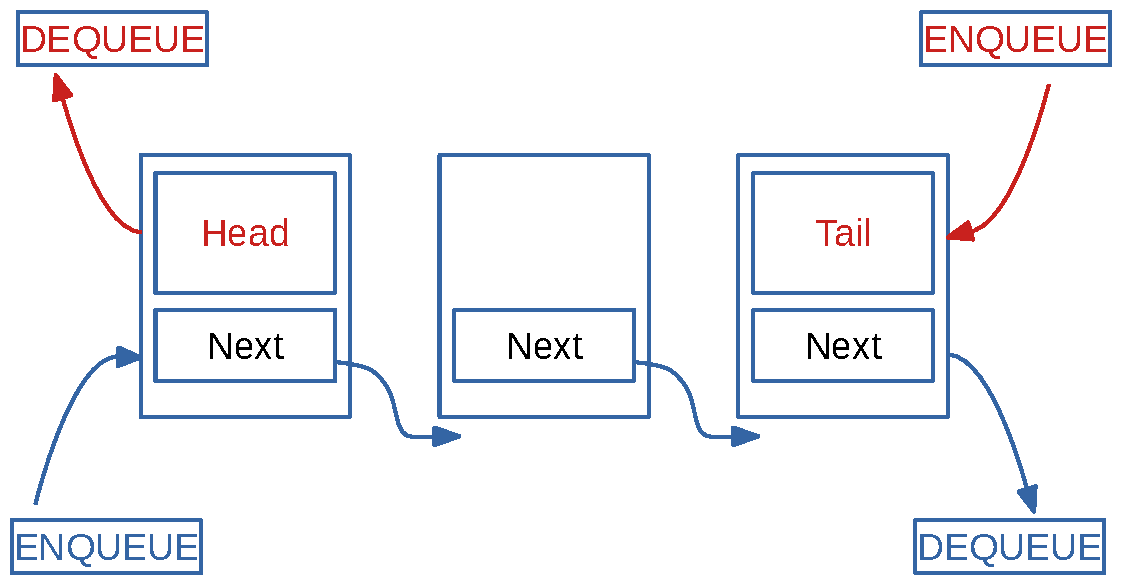
\includegraphics[scale=.6]{chapters/datastructures/images/queue_2.pdf}
		\caption[In a deque the operations can be done on both head and tail.]{In a deque the operations can be done on both head and tail.}
		\label{queue_2}
	\end{center}
\end{figure}

\begin{figure}[H]
\centering
\begin{tikzpicture}[draw, minimum width=1.5cm, minimum height=0.5cm, thick]  
    \node[draw] (enqueue) at (-1.5,2) {};
    \node[draw=none] at ($(enqueue) + (0, 5mm)$) {Enqueue $O(1)$};
    \node[draw] (dequeue1) at (1.5,2) {};
    \node[draw=none] at ($(dequeue1) + (0, 5mm)$) {Dequeue $O(1)$};
    
    \node[draw] (dequeue) at (1.5,-2) {};
    \node[draw=none] at ($(dequeue) + (0, -5mm)$) {Dequeue $O(1)$};
    \node[draw] (enqueue1) at (-1.5,-2) {};
    \node[draw=none] at ($(enqueue1) + (0, -5mm)$) {Enqueue $O(1)$};
    
    \matrix (queue)[matrix of nodes, nodes={draw, nodes={draw}}, nodes in empty cells, row sep=-\pgflinewidth]
    {
      Head \\ 
       \\ 
       \\ 
       Tail \\
    };

    \draw[->, >=stealth] (0.25,-1.052) -- (dequeue.north);
    \draw[->, >=stealth] (enqueue.south) -- (-0.25,1.05);
    
    \draw[->, >=stealth] (enqueue1.north) -- (-0.25,-1.05);
    \draw[->, >=stealth] (0.25,1.05) -- (dequeue1.south);
\end{tikzpicture}
\caption[In a deque the operations can be done on both head and tail.]{In a deque the operations can be done on both head and tail.}
\label{queue_2}
\end{figure}

Another modification of queue are \textbf{priority queue}, in which each element has a priority (a numeric value that indicates its importance). When an element of the queue is removed (deque), the element to be removed is the one which has the highest priority. In case two or more elements have the same priority the oldest element is removed.

\begin{figure}[H]
	\begin{center}
		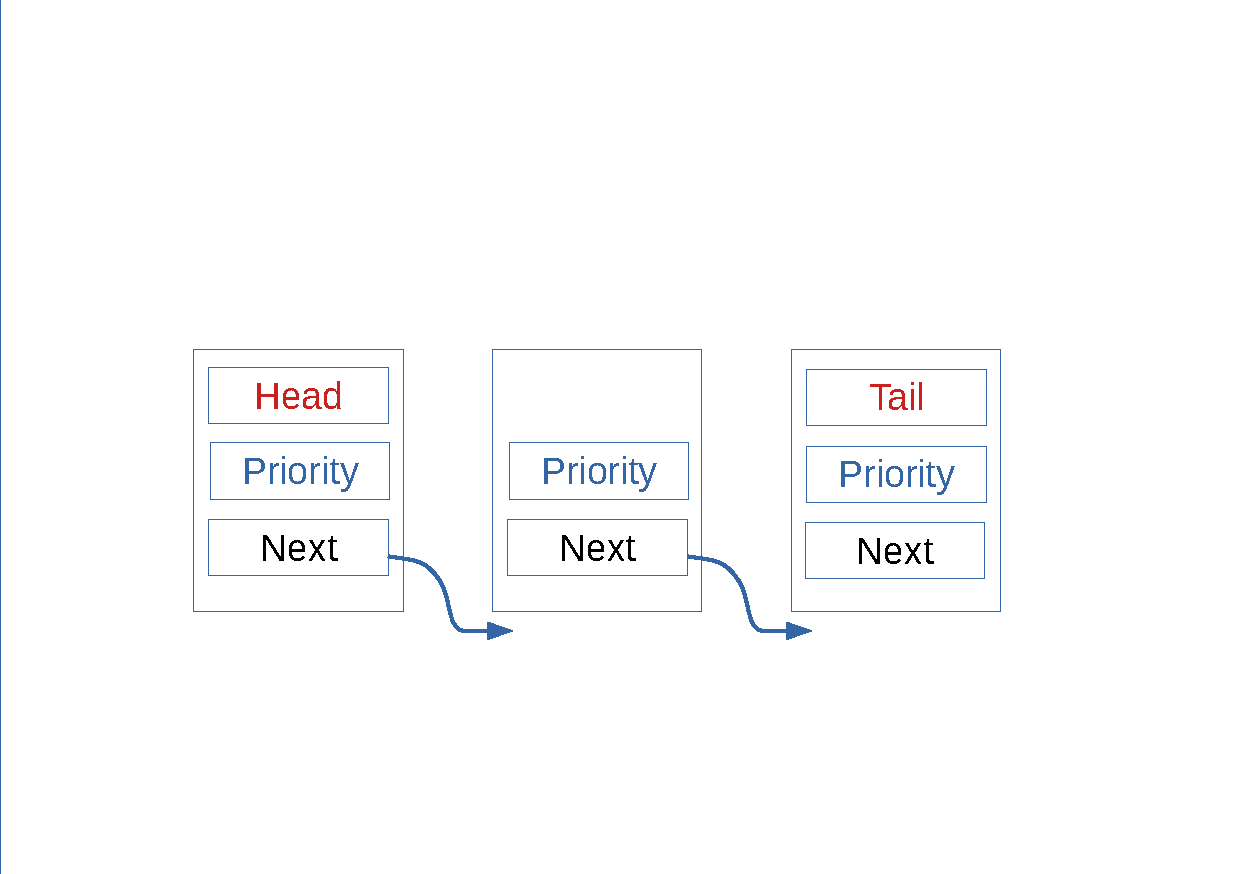
\includegraphics[scale=.6]{chapters/datastructures/images/queue_3.pdf}
		\caption[A priority queue.]{A priority queue.}
		\label{queue_3}
	\end{center}
\end{figure}

\begin{figure}[H]
\centering
\begin{tikzpicture}[draw, minimum width=2.7cm, minimum height=0.5cm, thick]  

    \matrix (queue)[matrix of nodes, nodes={draw, nodes={draw}}, nodes in empty cells, row sep=-\pgflinewidth]
    {
      Head, Priority \\ 
       \\
       \\
       \\
      Tail, Priority \\
    };

\end{tikzpicture}
\caption[A priority queue.]{A priority queue.}
\label{queue_3}
\end{figure}

\subsection{Queue Implementation}
The following is the implementation of a queue using the list of Python.
\begin{lstlisting}[firstnumber=1, caption={Queue implementation.}]
class Queue():
	def __init__(self, head=None):
		self.storage = [head]
	
	def enqueue(self, new_element):
		self.storage.append(new_element)
	
	def peek(self):
		return self.storage[0]
	
	def dequeue(self):
		return self.storage.pop(0)
\end{lstlisting}

\section{Set}
A \textbf{set} is an abstract data type in which the unique values are stored without a particular order \cite{wikiset} (\href{https://en.wikipedia.org/wiki/Set_(abstract_data_type)}{Set, Wikipedia}).

\section{Map}
A \textbf{map}, \textbf{associative array}, \textbf{symbol table}, or \textbf{dictionary} is an abstract data type composed of a collection of (key, value) pairs \cite{wikihashmap} (\href{https://en.wikipedia.org/wiki/Associative_array}{Hash Map, Wikipedia}). The group of the key is a set, in which each element has a unique value. Map is a very useful data type, used in a lot of situations. 

\begin{figure}[H]
	\begin{center}
		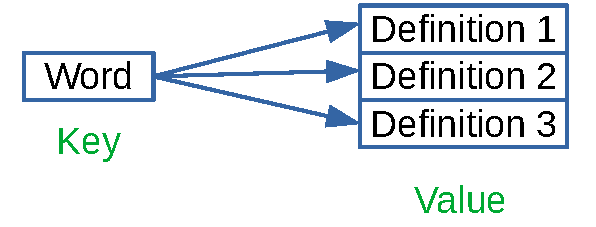
\includegraphics[scale=.6]{chapters/datastructures/images/map_1.pdf}
		\caption[An example of a map.]{An example of a map.}
		\label{map_1}
	\end{center}
\end{figure}

\begin{figure}[H]
\centering
\begin{tikzpicture}[draw, minimum width=2.4cm, minimum height=0.5cm, thick]  

    \matrix [matrix of nodes, nodes={draw, nodes={draw}}, nodes in empty cells, row sep=-\pgflinewidth] (queue)
    {
      Definition $1$ \\ 
      Definition $2$ \\
      Definition $3$ \\
    };
    
    \node[rectangle, draw, minimum width=1cm, minimum height=0.5cm] (word) at ($(queue) + (-3.6,0)$) {Word};
    
    \node[draw=none] (key) at ($(word) + (0,-8mm)$) {\textcolor{ForestGreen}{Key}};
    \node[draw=none] (key) at ($(queue) + (0,-14mm)$) {\textcolor{ForestGreen}{Value}};
    
    \draw[->, >=stealth] (word.east) -- (queue-1-1.west);
    \draw[->, >=stealth] (word.east) -- (queue-2-1.west);
	\draw[->, >=stealth] (word.east) -- (queue-3-1.west);    
    
\end{tikzpicture}
\caption[An example of a map.]{An example of a map.}
\label{map_1}
\end{figure}

\section{Hash Table}
A \textbf{hash table} or \textbf{hash map} is a data structure that implements the map abstract data type \cite{wikihashtable} (\href{https://en.wikipedia.org/wiki/Hash_table}{Hash Table, Wikipedia}). Hash table uses the \textbf{hash function} for working \cite{wikihashfunction} (\href{https://en.wikipedia.org/wiki/Hash_function}{Hash Function, Wikipedia}). Using the hash function is called hashing.

\subsection{Hashing}
Hashing is an operation that allows to transform the value of a variable to another one which is much easier to find within a collection. If we want to find a value inside a collection (list, stack, queue, etc) the time requested for the search is linear with the size of the collection. In fact we have to check all the elements until the searched one is found (in case of stack and queue this is not true is only the last or the first element respectively is checked). For solving this problem and thus to find an element in a constant time hash function are used. 

Let us consider the follow example, where we have an array in which we would like to store big random numbers. A simple way for hashing these numbers is to consider only the last numbers (56 and 17) and divide them for a fixed number. The reminder of the division is used as the new index of the array associated to the number (Figure ).

What happen when the hash function transforms two different number in the same? In this case we have a \textbf{collision}. In case of a collision there are several strategies for solving this issue: one way could be to change the the hash function, another one could be to use an array for storing different values associated to the same key (\textbf{bucket}). For the last occurrence the worst case complexity for a search is \(O(n)\) (Figure \ref{map_2}).

\begin{figure}[H]
	\begin{center}
		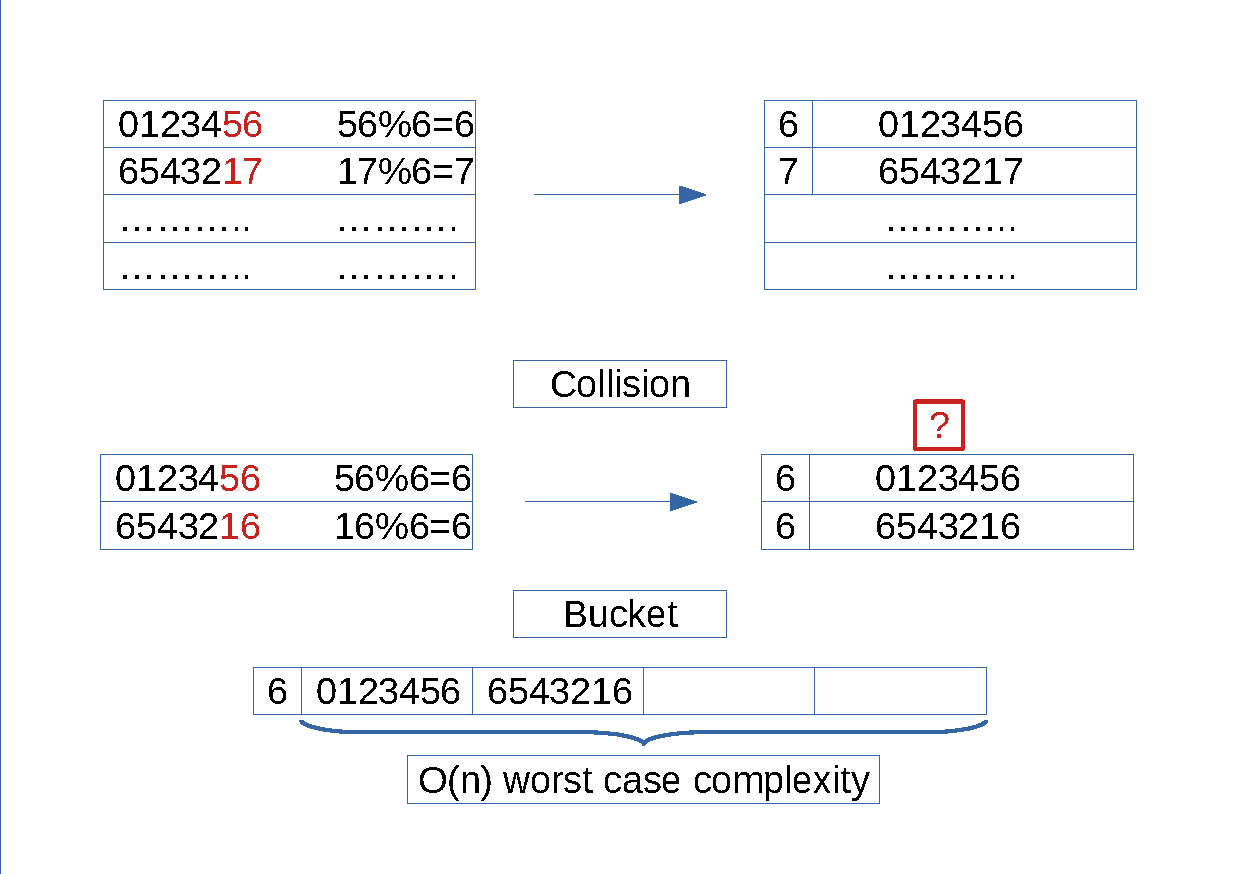
\includegraphics[scale=.6]{chapters/datastructures/images/map_2.pdf}
		\caption[An example of collision and a possible way to solve this issue by using the bucket method.]{An example of collision and a possible way to solve this issue by using the bucket method.}
		\label{map_2}
	\end{center}
\end{figure}

\begin{figure}[H]
\centering
\begin{tikzpicture}[draw, minimum width=4.2cm, minimum height=0.5cm, thick, align=center]  

    \matrix [matrix of nodes, nodes={draw, nodes={draw}}, nodes in empty cells, row sep=-\pgflinewidth] (tab1)
    {
      $01234\textcolor{BrickRed}{56} \qquad 56\%6=6$ \\ 
      $65432\textcolor{BrickRed}{17} \qquad 17\%6=7$ \\
      ... \qquad ... \\
      ... \qquad ... \\
    };
    
    \matrix [matrix of nodes, nodes={draw, nodes={draw}}, nodes in empty cells, row sep=-\pgflinewidth, minimum width=3cm, minimum height=0.5cm] (tab2) at ($(tab1) + (7.6,0)$)
    {
      $6 -> 0123456$ \\ 
      $7 -> 6543217$ \\
      ... \qquad ... \\
      ... \qquad ... \\
    };
    
    \draw[->, >=stealth] (tab1) -- (tab2);
    
    
    \draw (3.6,-2) node[draw=none, rectangle, align=left] (collision) {Collision};
    
    \matrix [matrix of nodes, nodes={draw, nodes={draw}}, nodes in empty cells, row sep=-\pgflinewidth] (tab3) at ($(tab1) + (0,-3)$)
    {
      $01234\textcolor{BrickRed}{56} \qquad 56\%6=6$ \\ 
      $65432\textcolor{BrickRed}{16} \qquad 16\%6=6$ \\
    };
    
    \matrix [matrix of nodes, nodes={draw, nodes={draw}}, nodes in empty cells, row sep=-\pgflinewidth, minimum width=3cm, minimum height=0.5cm] (tab4) at ($(tab3) + (7.6,0)$)
    {
      $6 -> 0123456$ \\ 
      $6 -> 6543216$\\
    };
    \draw ($(tab4.north) + (0,2mm)$) node[draw, rectangle, align=left, BrickRed, minimum width=0.5cm, minimum height=0.5cm] {?};
    
    \draw[->, >=stealth] (tab3) -- (tab4);
    
    \draw (3.6,-4) node[draw=none, rectangle, align=left] {Bucket};
        
    \matrix [matrix of math nodes, nodes={draw, nodes={draw}, anchor=center}, nodes in empty cells, row sep=-\pgflinewidth, minimum width=0.5cm, minimum height=0.6cm, column sep=-\pgflinewidth] (tab5) at ($(tab3) + (3.6,-1.6)$)
    {
      $6$ & $0123456$ & $6543216$ & ... & $n$ \\
    };
    \draw ($(tab5) + (0,-7mm)$) node[draw=none, rectangle, align=left]  {$O(n)$ worst case complexity};

\end{tikzpicture}
\caption[An example of collision and a possible way to solve this issue by using the bucket method.]{An example of collision and a possible way to solve this issue by using the bucket method.}
\label{map_2}
\end{figure}

It does not exist a perfect hash function and a trade off must always be reached. A way to analyse a hash function is by using the \textbf{load factor} defined as follow: \(Load \ Factor = \# \ of \ entries / \ \# \ of \ buckets\). For example, if we want to save 10 values using 1000 buckets the Load Factor is equal to 0.01, and most of the buckets is empty. In this case is convenient to change the hash function by using less buckets. More the Load Factor is closed to 0 more the hash table will be empty (\textbf{sparse}), and more the Load Factor is closed to 1 more the has table will be full and efficient. In case the Load Factor is bigger than 1 there is the certainty there will happen some collisions.
Another example: let us consider a hash function that divide the numbers by 100. If we consider 100 values all multiple of 5, the Load Factor will be: \(Load \ Factor = \# \ of \ entries / \ \# \ of \ buckets = 100/100 = 1\). But this way is very slow and a different configuration should be used to make this more efficient. For example if we use more bucket, for example 107, we still avoid collisions and we do not have the hash map too much sparse.

\section{String Keys}
Let us consider a hash function that associates a word to a numerical value. For example we can use the ASCII character encoding of the first two letters of the string as numerical value. Thus, in case of \textit{UDACIY} we have \textit{U}=85 and \textit{D}=68. For hash function we can use the following: \(S\left[0\right] * 31^{(n-1)} + S\left[1\right] * 31^{(n-2)} + \ldots + S\left[n-1\right]\), where \(n\) is the length of the string. In this way for the word in the previous example, in which only the first two letters are encoded in a numerical value for simplicity, we have \(85*31^{1} + 68 = 2703\).

This hash function works very well because it assures a very low probability of collision. \(31\) is a number empirically obtained by several researches and showed good results in hashing strings.

\subsection{String Keys Implementation}
The following is the implementation of the string key map in Python.

The hash function of this implementation is: \(Hash \ Function = (ASCII[0]*100) + ASCII[1]\). In this code \textit{ord()} and \textit{char()} functions are used. \textit{ord()} takes a char as an argument and return the respective ASCII code (\(ord('U')=85\)), and \textit{char()} takes a numeric value as ASCII code and return the respective char (\(char(85)='U'\)).
\begin{lstlisting}[firstnumber=1, caption={String key implementation.}]
class HashTable():
	def __init__(self):
		self.table = [None]*10000
	
	def store(self, string):
		hv = self.calculate_hash_value(string)
		if hv != -1:
			if self.table[hv] != None:
				self.table[hv].append(string)
			else:
				self.table[hv] = [string]
	
	def lookup(self, string):
		hv = self.calculate_hash_value(string)
		if hv != -1:
			if self.table[hv] != None:
				if string in self.table[hv]:
					return hv
		return -1
	
	def calculate_hash_value(self, string):
		value = ord(string[0]*100) + ord(string[1])
		return value
\end{lstlisting}
\chapter{Searching and Sorting}
\label{chp: searchandsorting}
In this chapter are introduced the most important and used algorithms about \textbf{searching}, which retrieve some data stored in a particular data structure \cite{wikisearch} (\href{https://en.wikipedia.org/wiki/Search_algorithm}{Search algorithm, Wikipedia}), and \textbf{sorting}, which put in a certain order some data stored in a list \cite{wikisorting} (\href{https://en.wikipedia.org/wiki/Sorting_algorithm}{Sorting algorithm, Wikipedia}).
\section{Binary Search}
Let us consider the problem of finding a number stored in an array with an \textbf{ascending} order (Figure \ref{sorting_1}).

\begin{figure}[H]
	\begin{center}
		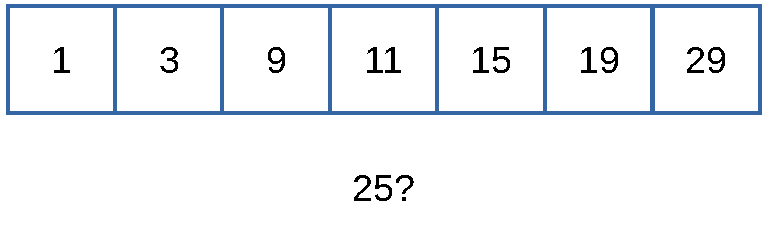
\includegraphics[scale=.6]{chapters/searchandsorting/images/sorting_1.pdf}
		\caption[An array with numeric values ordered in an ascending order.]{An array with numeric values ordered in an ascending order.}
		\label{sorting_1}
	\end{center}
\end{figure}

\begin{figure}[H]
\centering
\tikzset{
mymat/.style={
  matrix of math nodes,
  text height=2.5ex,
  text depth=0.75ex,
  text width=3.25ex,
  align=center,
  column sep=-\pgflinewidth
  },
mymats/.style={
  mymat,
  nodes={draw,fill=#1}
  }  
}
\begin{tikzpicture}[node distance = 5mm and 0mm,
start chain = A going right,
box/.style = {rectangle, draw, inner sep=1mm, outer sep=0mm,
              minimum size=7mm,
                 on chain=A},
LA/.style = {-{Straight Barb[flex=0]},
               thick, shorten >=1mm, shorten <=1mm,
               looseness=1.6}, >=latex, nodes in empty cells, thick]

\matrix[mymat, anchor=east, row 1/.style={nodes=draw} ] (mat1)
{
1 & 3 & 9 & 11 & 15 & 19 & 29 \\
};

\draw ($(mat1.south) + (0,-4mm)$) node[draw=none, rectangle, align=left] {$25?$};

\end{tikzpicture}
\caption[An array with numeric values ordered in an ascending order.]{An array with numeric values ordered in an ascending order.}
\label{sorting_1}
\end{figure}

A first way to tackle the problem could be to check all the numbers of the array, in others words this method consists in performing a loop all over the elements of the array and check one by one if the number where is the element we are looking for. The complexity of this method is \(O(n)\) because in the worst case we have to look at all the elements of the array. 

There is a more efficient way to search an element in an ascending ordered array then the method showed previously. This method is called \textbf{binary search} \cite{wikibinarysearch} (\href{https://en.wikipedia.org/wiki/Binary_search_algorithm}{Binary Search Algorithm, Wikipedia}).
Let us start to check as the first element the central value of the array (in case the array has an even number of elements there are two central values, and one can choose the bigger or the lower). If the central element is the one we are looking for the search ends, otherwise, because the array is ascending ordered, we can ignore one half of the array. If the central number is bigger than the number we are looking for thus we will ignore the right half of the array, if the central number is lower than the number we are looking for thus we will ignore the left half of the array. This procedure is repeated: we consider the central value of the new array, which has half of the size of the previous step, and we check is that value is the one we are looking for, and we repeat the procedure until or we find or we do not find the number we are looking for (Figure \ref{sorting_2}). 

\begin{figure}[H]
	\begin{center}
		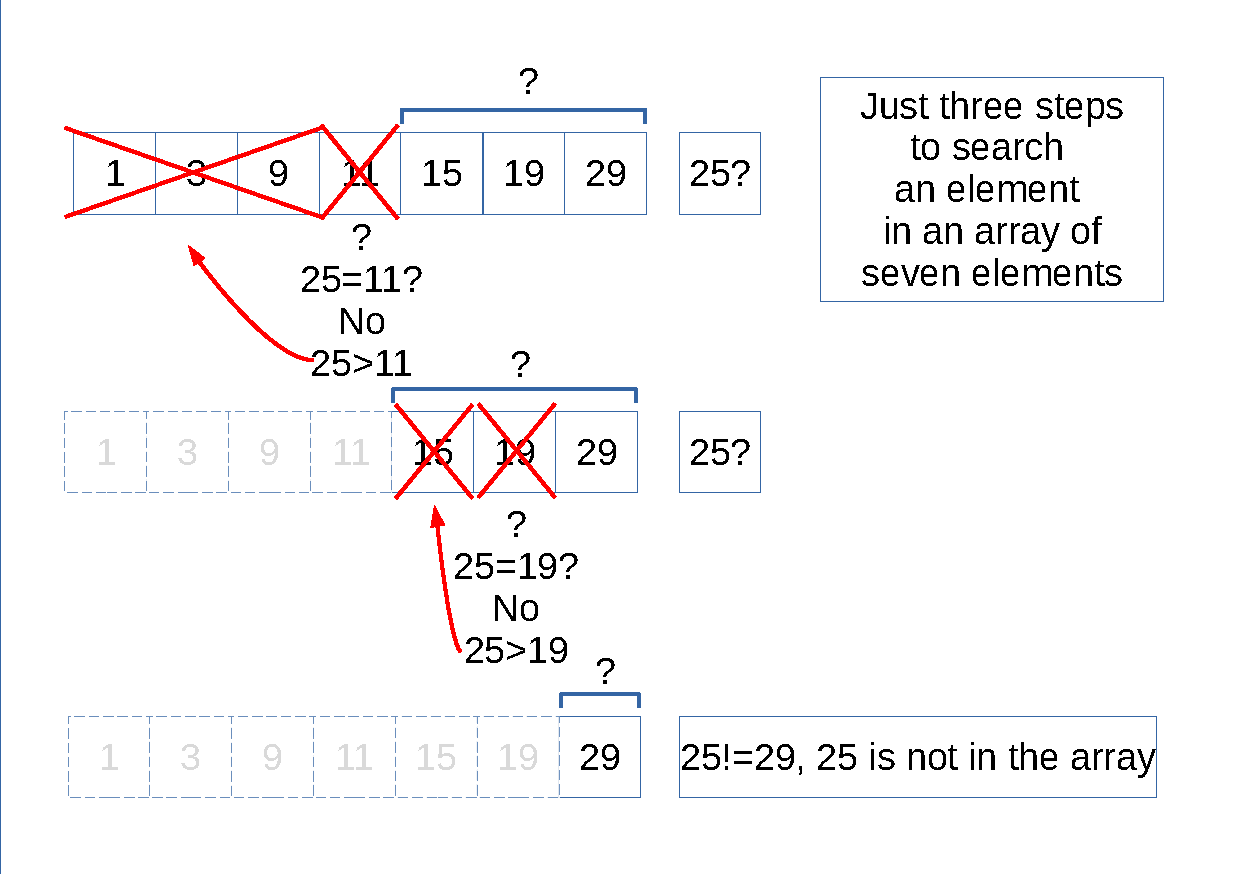
\includegraphics[scale=.6]{chapters/searchandsorting/images/sorting_2.pdf}
		\caption[Binary search algorithms steps.]{Binary search algorithms steps.}
		\label{sorting_2}
	\end{center}
\end{figure}

\begin{figure}[H]
\centering
\begin{tikzpicture}[font=\ttfamily,
array/.style={matrix of nodes,nodes={draw, minimum size=7mm},column sep=-\pgflinewidth, row sep=0.5mm, nodes in empty cells}, thick]

\matrix[array, nodes={fill=ForestGreen!30}, row 1 column 4/.style={nodes={fill=BrickRed!30}}] (array1) {
1 & 3 & 9 & 11 & 15 & 19 & 29 \\};
\draw ($(array1.east) + (10mm,0)$) node[draw, rectangle, align=left, minimum size=7mm] {$25>11$};

\matrix[array, fill=none, row 1 column 5/.style={nodes={fill=ForestGreen!30}}, row 1 column 6/.style={nodes={fill=BrickRed!30}}, row 1 column 7/.style={nodes={fill=ForestGreen!30}}] (array2) at ($(array1) + (0, -14mm)$){
1 & 3 & 9 & 11 & 15 & 19 & 29 \\};
\draw ($(array2.east) + (10mm,0)$) node[draw, rectangle, align=left, minimum size=7mm] {$25>19$};
\draw[->, >=stealth, BrickRed] (array1-1-4) -- (array2-1-4);

\matrix[array, fill=none, row 1 column 7/.style={nodes={fill=BrickRed!30}}] (array3) at ($(array2) + (0, -14mm)$){
1 & 3 & 9 & 11 & 15 & 19 & 29 \\};
\draw ($(array3.east) + (25.2mm,0)$) node[draw, rectangle, align=left, minimum size=7mm] {$25\neq19$ \\ 25 is not in the array};
\draw[->, >=stealth, BrickRed] (array2-1-6) -- (array3-1-6);

\end{tikzpicture}

\caption[Binary search algorithms steps.]{Binary search algorithms steps.}
\label{sorting_2}
\end{figure}

\subsection{Efficiency of the Binary Search Algorithm}
For evaluating the efficiency of this algorithm we have to evaluate the number of steps required for solving the problem. We already know that the efficiency of this algorithm will not be \(O(n)\), because in this algorithm not all the elements of the array are checked. The way for evaluating the complexity of an algorithm is to execute the algorithms varying the size of the input, and evaluating how many operations are done in the worst case. In the binary search algorithm the worst case is when the size of the array becomes one, so we find or we do not find the searched element at the end of the array splitting process.

\begin{table}[H]
\caption[Binary Search Efficiency.]{The number of iterations grows of one every power of two, in others words it grows as \(log(n)\).}
\label{binarysearchefficiency}
\centering
\begin{tabular}{ | l | c | c | c | c | c | c | c | c | c |}
   
    \multicolumn{1}{l}{} & \multicolumn{1}{c}{} & 
    \multicolumn{1}{c}{\(2^{0}\)} & \multicolumn{1}{c}{\(2^{1}\)} &
    \multicolumn{1}{c}{} & \multicolumn{1}{c}{\(2^{2}\)} & 
    \multicolumn{1}{c}{} & \multicolumn{1}{c}{}          & 
    \multicolumn{1}{c}{} & \multicolumn{1}{c}{\(2^{3}\)} \\
    \hline
	Array Size & 0 & \cellcolor{LightCyan} 1 & \cellcolor{LightCyan} 2 & 3 & \cellcolor{LightCyan} 4  & 5 & 6 & 7 & \cellcolor{LightCyan} 8 \\
    \hline
	Iterations (worst case) & 0 & \cellcolor{LightCyan} 1 & \cellcolor{LightCyan} 2 & 2 & \cellcolor{LightCyan} 3 & 3 & 3 & 3 & \cellcolor{LightCyan} 4 \\
	\hline	
\end{tabular}
\end{table}

We observe that the exponent of the power of two is the number of iteration minus one, or at the contrary the number of iteration is the exponent of a power plus one.
\begin{center}
\(log( power\ of\ exponent\ 2 + 1) = log_{2}(n) + 1\)
\end{center}
In general it is used \(log\) and is said that the binary search algorithm has a complexity of \(log(n)\). 

\subsection{Binary Search Implementation}
The following code is the python implementation of the binary search algorithm.
\begin{lstlisting}[firstnumber=1, caption={Binary search python implementation.}]
def binary_search(array_input, value):
	low = 0
	high = len(array_input) - 1
	while low <= high:
		mid = (low + high) // 2
		if array_input[mid] == value:
			return mid
		elif value > array_input[mid]:
			new_low = mid + 1
		else:
			new_high = mid - 1
	return -1
\end{lstlisting}

\begin{figure}[H]
	\begin{center}
		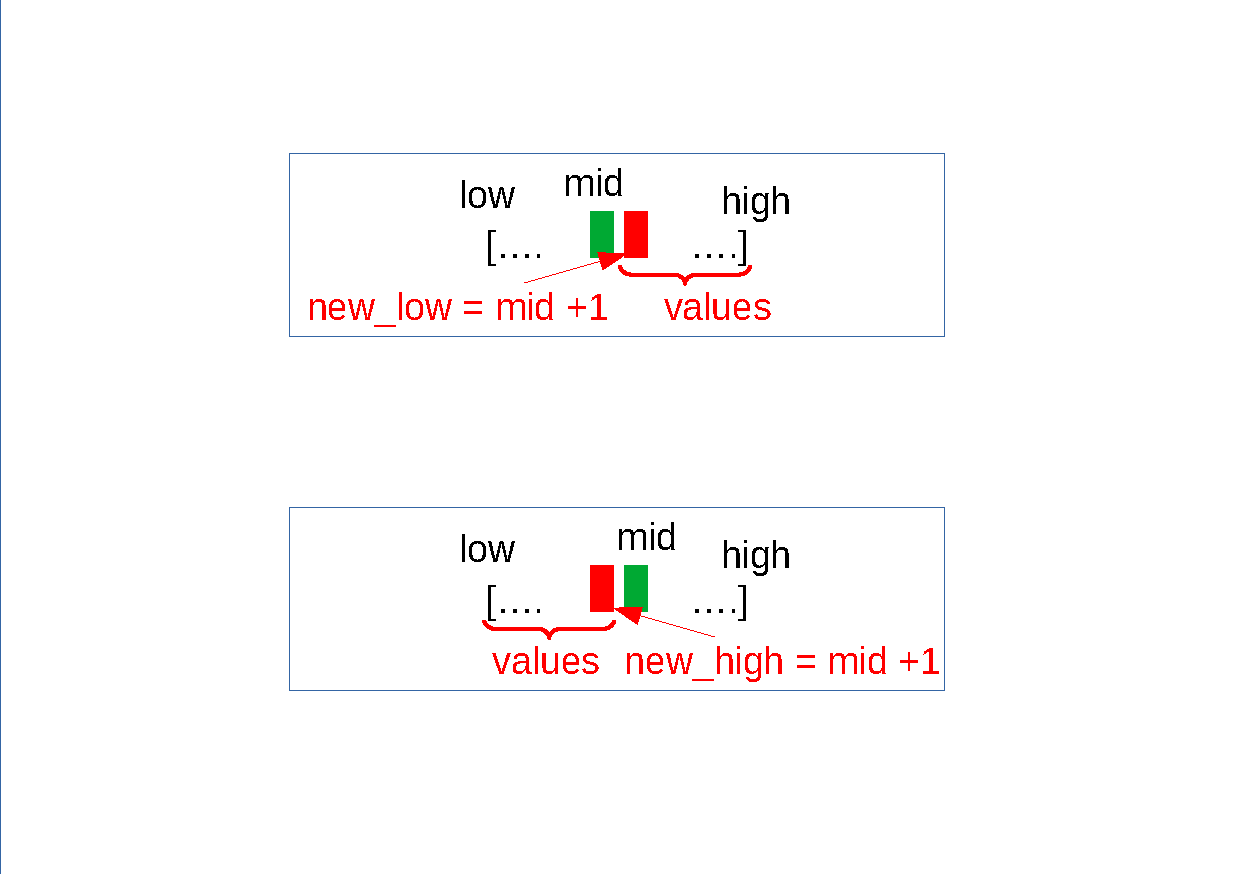
\includegraphics[scale=.6]{chapters/searchandsorting/images/sorting_3.pdf}
		\caption[Array splitting in the implementation of the binary search algorithm.]{Array splitting in the implementation of the binary search algorithm.}
		\label{sorting_3}
	\end{center}
\end{figure}

\begin{figure}[H]
\centering
\begin{tikzpicture}[font=\ttfamily,
array/.style={matrix of nodes,nodes={draw, minimum size=7mm},column sep=-\pgflinewidth, row sep=0.5mm, nodes in empty cells}, thick]

\matrix[array, fill=none, row 2 column 1/.style={nodes={fill=ForestGreen!30}}, row 2 column 7/.style={nodes={fill=ForestGreen!30}}, row 2 column 4/.style={nodes={fill=BrickRed!30}},
row 1/.style={nodes={draw=none, fill=none, minimum size=5mm}}] (array1) {
L &   &   & M  &    &    & H  \\ 
1 & 3 & 9 & 11 & 15 & 19 & 29 \\};

\matrix[array, fill=none, row 2 column 5/.style={nodes={fill=ForestGreen!30}}, row 2 column 6/.style={nodes={fill=BrickRed!30}}, row 2 column 7/.style={nodes={fill=ForestGreen!30}},
row 1/.style={nodes={draw=none, fill=none, minimum size=5mm}}] (array2) at ($(array1) + (0, -16mm)$){
  &   &   &    & L' & M  & H  \\
1 & 3 & 9 & 11 & 15 & 19 & 29 \\};
\draw ($(array2-2-7.east) + (12mm,0)$) node[draw, rectangle, align=left, minimum size=7mm] {L'=M+1};

\matrix[array, fill=none, row 2 column 1/.style={nodes={fill=ForestGreen!30}}, row 2 column 3/.style={nodes={fill=ForestGreen!30}}, row 2 column 2/.style={nodes={fill=BrickRed!30}},
row 1/.style={nodes={draw=none, fill=none, minimum size=5mm}}] (array3) at ($(array2) + (0, -16mm)$){
L & M & H' &    &    &    &   \\
1 & 3 & 9 & 11 & 15 & 19 & 29 \\};
\draw ($(array3-2-7.east) + (12mm,0)$) node[draw, rectangle, align=left, minimum size=7mm] {H'=M+-1};

\end{tikzpicture}

\caption[Array splitting in the implementation of the binary search algorithm.]{Array splitting in the implementation of the binary search algorithm.}
\label{sorting_3}
\end{figure}

\section{Bubble Sort}
\textbf{bubble sort} is the easiest sorting algorithm working on arrays. Bubble sort works by swapping two element at each step if they are in the wrong order, repeating this process until all the array is not completely ordered \cite{wikibubblesort} (\href{https://en.wikipedia.org/wiki/Bubble_sort}{Bubble Sort, Wikipedia}). In this algorithm the bigger elements tend to move at the bottom of the array, like bubbles that move at the top of a water bottle.

\begin{figure}[H]
	\begin{center}
		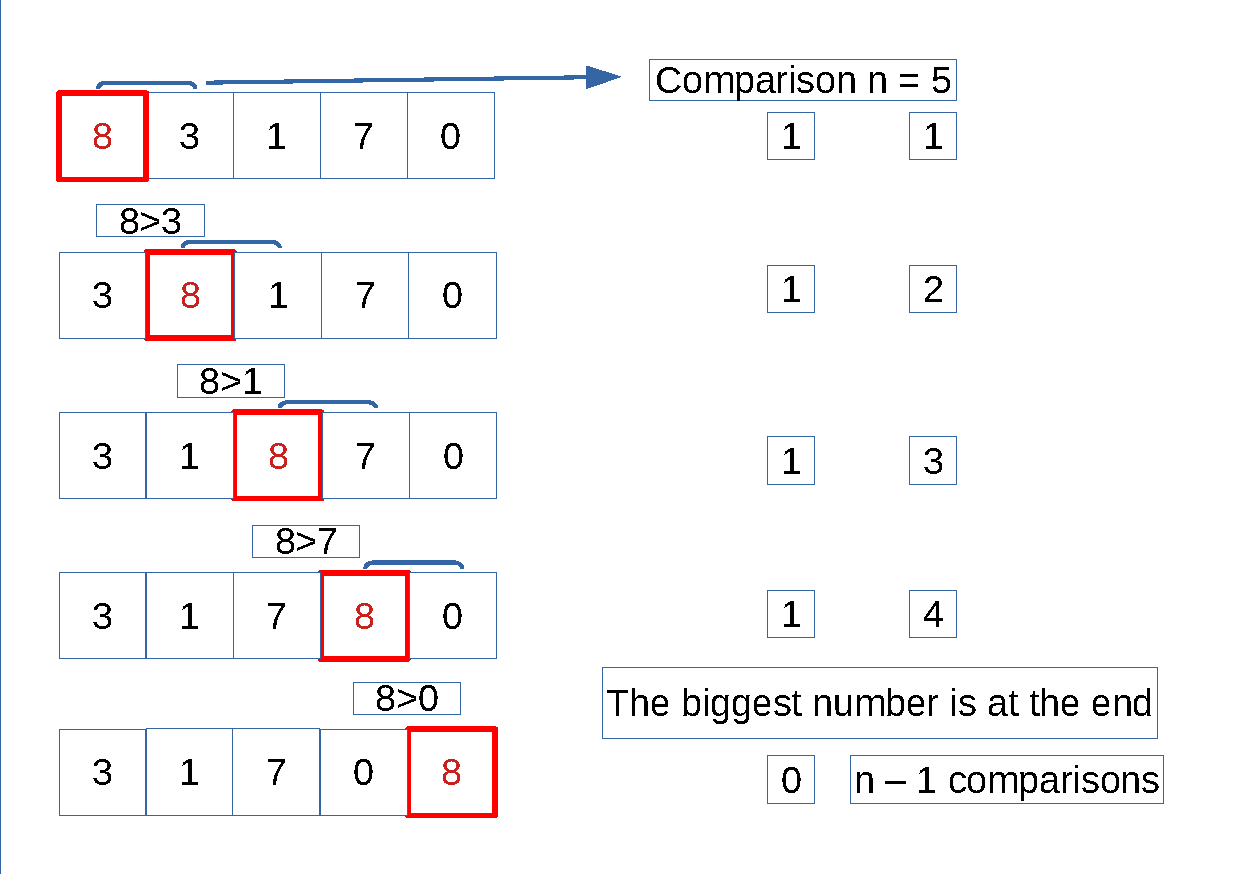
\includegraphics[scale=.6]{chapters/searchandsorting/images/sorting_4.pdf}
		\caption[Bubble sort algorithm.]{In bubble sort the biggest element goes at the and of the array.}
		\label{sorting_4}
	\end{center}
\end{figure}

\begin{figure}[H]
	\begin{center}
		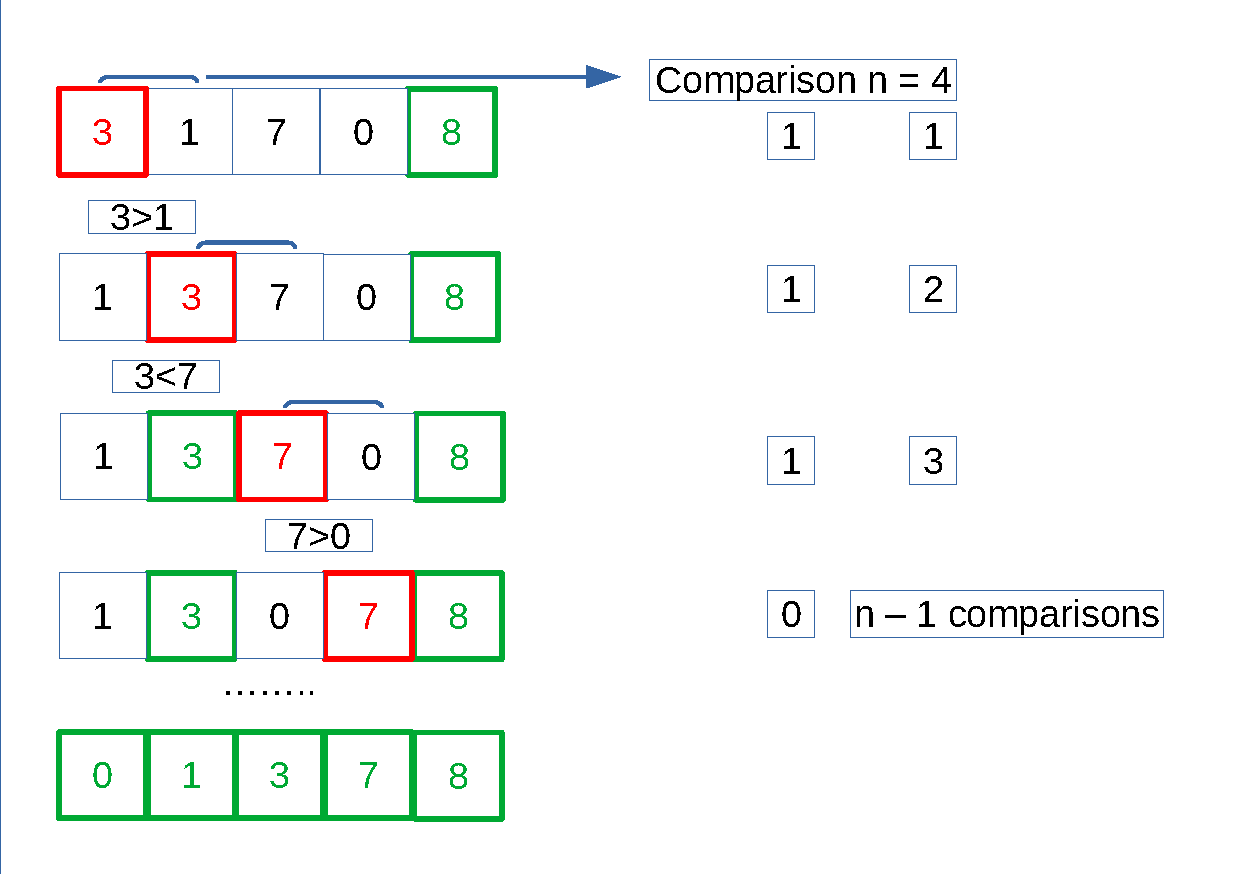
\includegraphics[scale=.6]{chapters/searchandsorting/images/sorting_5.pdf}
		\caption[The swapping process is repeated until the array is completely ordered.]{The swapping process is repeated until the array is completely ordered.}
		\label{sorting_5}
	\end{center}
\end{figure}

\begin{figure}[H]
\centering
\begin{tikzpicture}[font=\ttfamily,
array/.style={matrix of nodes,nodes={draw, minimum size=7mm},column sep=-\pgflinewidth, row sep=0.5mm, nodes in empty cells}, thick]

\matrix[array] (array1) {
8 & 3 & 1 & 7 & 0 \\};
\draw ($(array1.west) + (-14mm,0)$) node[draw=none, rectangle, align=left, minimum size=7mm, anchor=west] {Start};

\matrix[array, row 1 column 1/.style={nodes={fill=BrickRed!30}}] (array2) at ($(array1) + (0,-12mm)$) {
8 & 3 & 1 & 7 & 0 \\};
\draw ($(array2.west) + (-14mm,0)$) node[draw=none, rectangle, align=left, minimum size=7mm, anchor=west] {Step 1};
\draw ($(array2.east) + (20mm,0)$) node[draw=none, rectangle, align=center, minimum size=7mm, anchor=east] {Compare: \\ swap};
\path[<->, >=stealth, BrickRed] (array2-1-1.north) edge [bend left=40] (array2-1-2.north);

\matrix[array, row 1 column 2/.style={nodes={fill=BrickRed!30}}] (array3) at ($(array2) + (0,-12mm)$) {
3 & 8 & 1 & 7 & 0 \\};
\draw ($(array3.west) + (-14mm,0)$) node[draw=none, rectangle, align=left, minimum size=7mm, anchor=west] {Step 2};
\draw ($(array3.east) + (20mm,0)$) node[draw=none, rectangle, align=center, minimum size=7mm, anchor=east] {Compare: \\ swap};
\path[<->, >=stealth, BrickRed] (array3-1-2.north) edge [bend left=40] (array3-1-3.north);

\matrix[array, row 1 column 3/.style={nodes={fill=BrickRed!30}}] (array4) at ($(array3) + (0,-12mm)$) {
3 & 1 & 8 & 7 & 0 \\};
\draw ($(array4.west) + (-14mm,0)$) node[draw=none, rectangle, align=left, minimum size=7mm, anchor=west] {Step 3};
\draw ($(array4.east) + (20mm,0)$) node[draw=none, rectangle, align=center, minimum size=7mm, anchor=east] {Compare: \\ swap};
\path[<->, >=stealth, BrickRed] (array4-1-3.north) edge [bend left=40] (array4-1-4.north);

\matrix[array, row 1 column 4/.style={nodes={fill=BrickRed!30}}] (array5) at ($(array4) + (0,-12mm)$) {
3 & 1 & 7 & 8 & 0 \\};
\draw ($(array5.west) + (-14mm,0)$) node[draw=none, rectangle, align=left, minimum size=7mm, anchor=west] {Step 4};
\draw ($(array5.east) + (20mm,0)$) node[draw=none, rectangle, align=center, minimum size=7mm, anchor=east] {Compare: \\ swap};
\path[<->, >=stealth, BrickRed] (array5-1-4.north) edge [bend left=40] (array5-1-5.north);

\matrix[array, row 1 column 1/.style={nodes={fill=BrickRed!30}}] (array6) at ($(array5) + (0,-12mm)$) {
3 & 1 & 7 & 0 & 8 \\};
\draw ($(array6.west) + (-14mm,0)$) node[draw=none, rectangle, align=left, minimum size=7mm, anchor=west] {Step 5};
\draw ($(array6.east) + (20mm,0)$) node[draw=none, rectangle, align=center, minimum size=7mm, anchor=east] {Compare: \\ swap};
\path[<->, >=stealth, BrickRed] (array6-1-1.north) edge [bend left=40] (array6-1-2.north);

\matrix[array, row 1 column 2/.style={nodes={fill=BrickRed!30}}] (array7) at ($(array6) + (0,-12mm)$) {
1 & 3 & 7 & 0 & 8 \\};
\draw ($(array7.west) + (-14mm,0)$) node[draw=none, rectangle, align=left, minimum size=7mm, anchor=west] {Step 6};
\draw ($(array7.east) + (20mm,0)$) node[draw=none, rectangle, align=center, minimum size=7mm, anchor=east] {Compare: \\ no swap};
\path[<->, >=stealth, BrickRed] (array7-1-2.north) edge [bend left=40] (array7-1-3.north);

\matrix[array, row 1 column 3/.style={nodes={fill=BrickRed!30}}] (array8) at ($(array7) + (0,-12mm)$) {
1 & 3 & 7 & 0 & 8 \\};
\draw ($(array8.west) + (-14mm,0)$) node[draw=none, rectangle, align=left, minimum size=7mm, anchor=west] {Step 7};
\draw ($(array8.east) + (20mm,0)$) node[draw=none, rectangle, align=center, minimum size=7mm, anchor=east] {Compare: \\ swap};
\path[<->, >=stealth, BrickRed] (array8-1-3.north) edge [bend left=40] (array8-1-4.north);

\matrix[array, row 1 column 4/.style={nodes={fill=BrickRed!30}}] (array9) at ($(array8) + (0,-12mm)$) {
1 & 3 & 0 & 7 & 8 \\};
\draw ($(array9.west) + (-14mm,0)$) node[draw=none, rectangle, align=left, minimum size=7mm, anchor=west] {Step 8};
\draw ($(array9.east) + (20mm,0)$) node[draw=none, rectangle, align=center, minimum size=7mm, anchor=east] {Compare: \\ no swap};
\path[<->, >=stealth, BrickRed] (array9-1-4.north) edge [bend left=40] (array9-1-5.north);

\matrix[array, row 1 column 1/.style={nodes={fill=BrickRed!30}}] (array10) at ($(array9) + (0,-12mm)$) {
1 & 3 & 0 & 7 & 8 \\};
\draw ($(array10.west) + (-14mm,0)$) node[draw=none, rectangle, align=left, minimum size=7mm, anchor=west] {Step 9};
\draw ($(array10.east) + (20mm,0)$) node[draw=none, rectangle, align=center, minimum size=7mm, anchor=east] {Compare: \\ no swap};
\path[<->, >=stealth, BrickRed] (array10-1-1.north) edge [bend left=40] (array10-1-2.north);

\matrix[array, row 1 column 2/.style={nodes={fill=BrickRed!30}}] (array11) at ($(array10) + (0,-12mm)$) {
1 & 3 & 0 & 7 & 8 \\};
\draw ($(array11.west) + (-14mm,0)$) node[draw=none, rectangle, align=left, minimum size=7mm, anchor=west] {Step 10};
\draw ($(array11.east) + (20mm,0)$) node[draw=none, rectangle, align=center, minimum size=7mm, anchor=east] {Compare: \\ swap};
\path[<->, >=stealth, BrickRed] (array11-1-2.north) edge [bend left=40] (array11-1-3.north);

\matrix[array, row 1 column 3/.style={nodes={fill=BrickRed!30}}] (array12) at ($(array11) + (0,-12mm)$) {
1 & 0 & 3 & 7 & 8 \\};
\draw ($(array12.west) + (-14mm,0)$) node[draw=none, rectangle, align=left, minimum size=7mm, anchor=west] {Step 11};
\draw ($(array12.east) + (20mm,0)$) node[draw=none, rectangle, align=center, minimum size=7mm, anchor=east] {Compare: \\ no swap};
\path[<->, >=stealth, BrickRed] (array12-1-3.north) edge [bend left=40] (array12-1-4.north);

\matrix[array, row 1 column 1/.style={nodes={fill=BrickRed!30}}] (array13) at ($(array12) + (0,-12mm)$) {
1 & 0 & 3 & 7 & 8 \\};
\draw ($(array13.west) + (-14mm,0)$) node[draw=none, rectangle, align=left, minimum size=7mm, anchor=west] {Step 12};
\draw ($(array13.east) + (20mm,0)$) node[draw=none, rectangle, align=center, minimum size=7mm, anchor=east] {Compare: \\ swap};
\path[<->, >=stealth, BrickRed] (array13-1-1.north) edge [bend left=40] (array13-1-2.north);

\matrix[array] (array14) at ($(array13) + (0,-12mm)$) {
0 & 1 & 3 & 7 & 8 \\};
\draw ($(array14.west) + (-14mm,0)$) node[draw=none, rectangle, align=left, minimum size=7mm, anchor=west] {Step 13};
\draw ($(array14.east) + (20mm,0)$) node[draw=none, rectangle, align=center, minimum size=7mm, anchor=east] {Sorted};

\end{tikzpicture}

\caption[The swapping process is repeated until the array is completely ordered.]{The swapping process is repeated until the array is completely ordered.}
\label{sorting_4}
\end{figure}

\subsection{Efficiency of the Bubble Sort Algorithm}
For ordering an array using the bubble sort \(n - 1\) iterations are required, every step. The number of total steps are \(n - 1\), thus the total number of operations to be executed for ordering an array is \((n - 1)*(n - 1) = n^{2} - 2n + 1 = O(n^{2})\).
In summary:
\begin{itemize}
\item \textbf{Worst Case}: \(O(n^{2})\)
\item \textbf{Average Case}: \(O(n^{2})\)
\item \textbf{Best Case}: \(O(n)\). The array is already completely ordered and it is enough to cycle all the elements.
\end{itemize} 

\subsection{Bubble Sort Implementation}
The following code is the python implementation of the bubble sort algorithm.
\begin{lstlisting}[firstnumber=1, caption={Bubble Sort python implementation}.]
def bubble_sort(array_input):
	index = len(array_input) - 1
	sorted = False
	
	while not sorted:
		sorted = True
		for i in range(0, index):
			if array_input[i] > array_input[i + 1]:
				sorted = False
				array_input[i], array_input[i + 1] = array_input[i + 1], array_input[i]
	return array_input
\end{lstlisting}

\section{Merge Sort}
The \textbf{merge sort} algorithm works by dividing the array in single elements at first, grouping and ordering all the elements two by two. After the first step we will have a lot of subarrays of two elements. The next step is to merge all these subarrays and to order the elements. The merging and ordering process is repeated until the array is unified again \cite{wikimergesort} (\href{https://en.wikipedia.org/wiki/Merge_sort}{Merge Sort, Wikipedia}).  This way of reducing a big problem in several smaller is called \textbf{Divide et impera} (Divide and conquer).

\begin{figure}[H]
	\begin{center}
		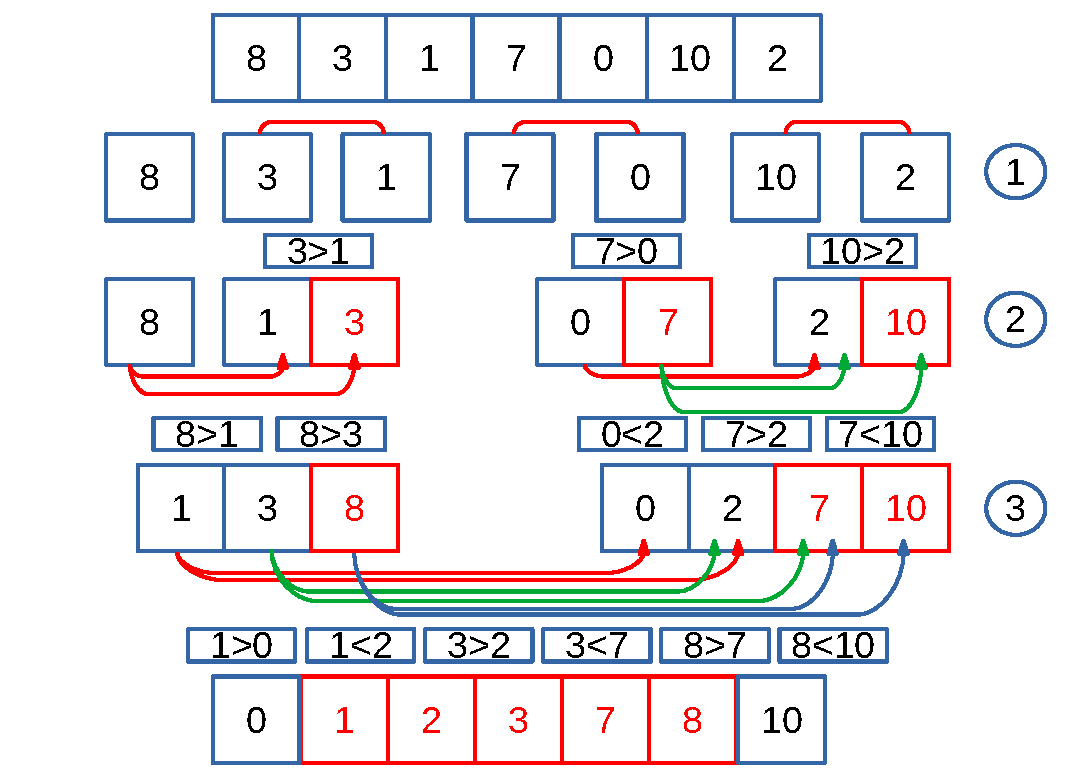
\includegraphics[scale=.52]{chapters/searchandsorting/images/sorting_6.pdf}
		\caption[Merge sort algorithm.]{In merge sort merging and sorting process is repeated until the array is again unified with all the elements sorted.}
		\label{sorting_6}
	\end{center}
\end{figure}

\begin{figure}[H]
\centering
\begin{tikzpicture}[font=\ttfamily,
array/.style={matrix of nodes,nodes={draw, minimum size=7mm},column sep=-\pgflinewidth, row sep=0.5mm, nodes in empty cells}, thick]

\matrix[array] (array11) {
8 & 3 & 1 & 7 & 0 & 10 & 2 \\};

\matrix[array] (array21) at ($(array11) + (-25mm, -14mm)$) {
8 & 3 & 1 & 7 \\};
\matrix[array] (array22) at ($(array11) + (25mm, -14mm)$){
0 & 10 & 2 \\};
\draw[->, >=stealth] (array11.south) -- (array21.north);
\draw[->, >=stealth] (array11.south) -- (array22.north);

\matrix[array] (array31) at ($(array21) + (-10mm, -14mm)$) {
8 & 3 \\};
\matrix[array] (array32) at ($(array21) + (10mm, -14mm)$){
1 & 7 \\};
\draw[->, >=stealth] (array21.south) -- (array31.north);
\draw[->, >=stealth] (array21.south) -- (array32.north);
\matrix[array] (array33) at ($(array22) + (-10mm, -14mm)$){
0 & 10 \\};
\matrix[array] (array34) at ($(array22) + (10mm, -14mm)$){
2 \\};
\draw[->, >=stealth] (array22.south) -- (array33.north);
\draw[->, >=stealth] (array22.south) -- (array34.north);

\matrix[array] (array41) at ($(array31) + (-5mm, -14mm)$) {
8 \\};
\matrix[array] (array42) at ($(array31) + (5mm, -14mm)$) {
3 \\};
\path[<->, >=stealth, BrickRed] ($(array41.south) + (0, 1.4mm)$) edge [bend right=40] ($(array42.south) + (0, 1.4mm)$);
\draw[->, >=stealth] (array31.south) -- (array41.north);
\draw[->, >=stealth] (array31.south) -- (array42.north);
\matrix[array] (array43) at ($(array32) + (-5mm, -14mm)$) {
1 \\};
\matrix[array] (array44) at ($(array32) + (5mm, -14mm)$) {
7 \\};
\draw[->, >=stealth] (array32.south) -- (array43.north);
\draw[->, >=stealth] (array32.south) -- (array44.north);
\matrix[array] (array45) at ($(array33) + (-5mm, -14mm)$) {
0 \\};
\matrix[array] (array46) at ($(array33) + (5mm, -14mm)$) {
10 \\};
\draw[->, >=stealth] (array33.south) -- (array45.north);
\draw[->, >=stealth] (array33.south) -- (array46.north);
\matrix[array] (array47) at ($(array34) + (0, -14mm)$) {
2 \\};
\draw[->, >=stealth] (array34.south) -- (array47.north);

\matrix[array] (array51) at ($(array31) + (0, -28mm)$) {
3 & 8 \\};
\matrix[array] (array52) at ($(array32) + (0, -28mm)$){
1 & 7 \\};
\path[->, >=stealth, BrickRed] ($(array51-1-1.south) + (0, 0)$) edge [bend right=40] ($(array52-1-1.south) + (0, 0)$);
\path[->, >=stealth, BrickRed] ($(array51-1-1.south) + (0, 0)$) edge [bend right=40] ($(array52-1-2.south) + (0, 0)$);
\path[->, >=stealth, BrickRed] ($(array51-1-2.north) + (0, 0)$) edge [bend left=40] ($(array52-1-1.north) + (0, 0)$);
\path[->, >=stealth, BrickRed] ($(array51-1-2.north) + (0, 0)$) edge [bend left=40] ($(array52-1-2.north) + (0, 0)$);
\draw[->, >=stealth] (array41.south) -- (array51.north);
\draw[->, >=stealth] (array42.south) -- (array51.north);
\draw[->, >=stealth] (array43.south) -- (array52.north);
\draw[->, >=stealth] (array44.south) -- (array52.north);
\matrix[array] (array53) at ($(array33) + (0, -28mm)$){
0 & 10 \\};
\matrix[array] (array54) at ($(array34) + (0, -28mm)$){
2 \\};
\draw[->, >=stealth] (array45.south) -- (array53.north);
\draw[->, >=stealth] (array46.south) -- (array53.north);
\draw[->, >=stealth] (array47.south) -- (array54.north);

\matrix[array] (array61) at ($(array21) + (0, -56mm)$) {
1 & 3 & 7 & 8 \\};
\matrix[array] (array62) at ($(array22) + (0, -56mm)$){
0 & 2 & 10 \\};
\draw[->, >=stealth] (array51.south) -- (array61.north);
\draw[->, >=stealth] (array52.south) -- (array61.north);
\draw[->, >=stealth] (array53.south) -- (array62.north);
\draw[->, >=stealth] (array54.south) -- (array62.north);

\matrix[array] (array71) at ($(array11) + (0, -84mm)$){
0 & 1 & 2 & 3 & 7 & 8 & 10 \\};
\draw[->, >=stealth] (array61.south) -- (array71.north);
\draw[->, >=stealth] (array62.south) -- (array71.north);

\end{tikzpicture}

\caption[Merge sort algorithm.]{In merge sort merging and sorting process is repeated until the array is again unified with all the elements sorted.}
\label{sorting_6}
\end{figure}

The steps are (Figure \ref{sorting_6}): 
\begin{itemize}
\item[1] Divide the array in subarryas of one element. Merge two by two and order the elements. The number of the subarrays is odd, so one array at this step is not merged. \textbf{The number of comparison for this step is 3}.
\item[2] Merge and order again the new subarrays. For ordering in this case we start from the first element of the array on the left, and we compare this value with all the elements of the array on the right. If the first element is bigger than the picked one from the array on the right is moved, otherwise is not moved and we go to the next element. \textbf{The number of comparison for this step is 5.}   
\item[3] Merge and order again as at the previous step. \textbf{The number of comparison for this step is 6.}
\end{itemize}

\subsection{Efficiency of the Merge Sort Algorithm}
For evaluating the efficiency of this algorithms we have to count the number of iterations and comparisons are being done. By using the example showed in Figure \ref{sorting_6} we will try to extrapolate a general pattern for an array of dimension \(n\).

The number of comparisons depends by the array size. For an array of two elements the number of comparisons is one, for one of three elements are two, for one of four are three, and for one of seven are six. It is impossible to calculate in general the number of comparisons, but it is possible to calculate the worst case given the array dimension. From the previous example we see that for each step the maximum number of comparisons is seven, the size of the array. The reason is that the sum of all subarrays is seven. In general the sum of all subarrays is always the size of the array. Thus the total efficiency is \(O(\# \ of\ comparison \ * \ \# \ of \ iterations \ )\).

How many iterations are required? In our example for an array of seven elements, the iterations required are three. From the subprocess of our example we observe that for an array of size four the number of iterations are two, for one of size three are two, and for one of size two is one. Thus we can create the following table:

\begin{table}[H]
\caption[Merge Sort Efficiency.]{The number of iterations grows of one every power of two, in others words it grows as \(log(n)\).}
\label{mergesortefficiency}
\centering
\begin{tabular}{ | l | c | c | c | c | c | c | c | c | c |}
   
    \multicolumn{1}{l}{} & \multicolumn{1}{c}{\(2^{0}\)} & 
    \multicolumn{1}{c}{\(2^{1}\)} & \multicolumn{1}{c}{} &
    \multicolumn{1}{c}{\(2^{2}\)} & \multicolumn{1}{c}{} & 
    \multicolumn{1}{c}{} & \multicolumn{1}{c}{}          & 
    \multicolumn{1}{c}{\(2^{3}\)} & \multicolumn{1}{c}{} \\
    \hline
	Array Size & \cellcolor{LightCyan} 1 & \cellcolor{LightCyan} 2 & 3 & \cellcolor{LightCyan} 4 & 5  & 6 & 7 & \cellcolor{LightCyan} 8 & 9 \\
    \hline
	Iterations (worst case) & \cellcolor{LightCyan} 0 & \cellcolor{LightCyan} 1 & 2 & \cellcolor{LightCyan} 2 & 3 & 3 & 3 & \cellcolor{LightCyan} 3 & 4 \\
	\hline	
\end{tabular}
\end{table}

In conclusion the efficiency if \(O(n \ log(n))\), which is better than \(O(n^{2})\) of the bubble sort. 

The memory efficiency in this case is bigger than the bubble sort algorithm. For the merge sort some subarrays (in the worst case are \(n\)) are used and they need to be stored in the memory.

\subsection{Merge Sort Implementation}
The following code is the python implementation of the merge sort algorithm.
\begin{lstlisting}[firstnumber=1, caption={Merge Sort python implementation.}]
def merge_sort(array_input):
	
	if len(array_input) > 1:
		mid = len(array_input)//2
		left_side = array_input[:mid]
		right_side = array_input[mid:]
		
		merge_sort(left_side)
		merge_sort(right_side)
		
		i = 0 # Left side index
		j = 0 # Right side index
		k = 0 # Sorted array index
		
		while i < len(left_side) and j < len(right_side):
			if left_side[i] < right_side[j]:
				array_input[k] = left_side[i]
				i+= 1
			else:
				array_input[k] = right_side[j]
				j+= 1
			k+= 1
			
		# Adding all elements if some of 
        # them have been left behind 
        while i < len(left_side): 
        	array_input[k] = left_side[i] 
            i+= 1
            k+= 1
            
        while j < len(right_side): 
        	array_input[k] = right_side[j] 
            j+= 1
            k+= 1
			
	return array_input
\end{lstlisting}

\begin{figure}[H]
	\begin{center}
		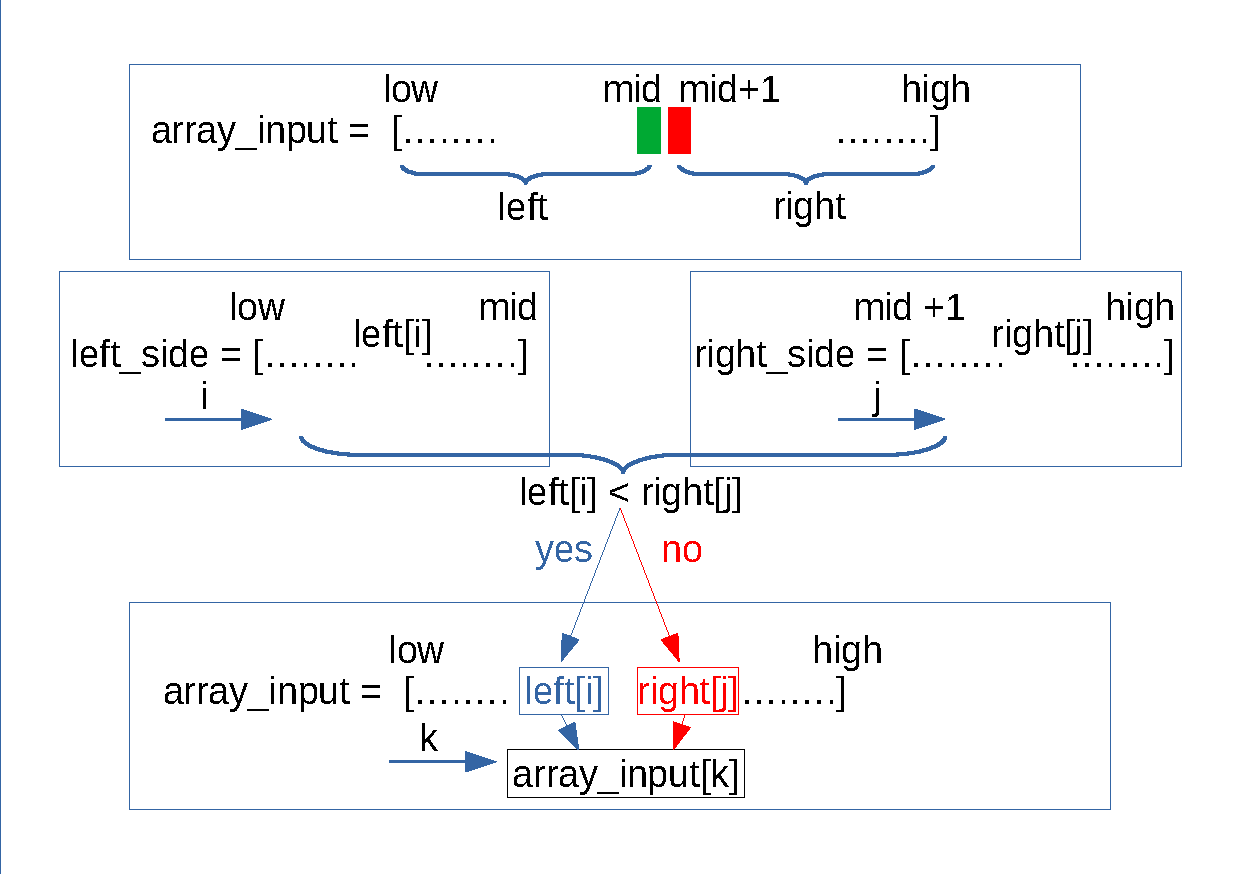
\includegraphics[scale=.6]{chapters/searchandsorting/images/sorting_7.pdf}
		\caption[Merge sort algorithm implementation.]{Merge sort algorithm implementation.}
		\label{sorting_7}
	\end{center}
\end{figure}

\section{Quicksort}
The \textbf{quicksort} is a sorting algorithm of the divide et impera type. It works by randomly choosing an element of the array, called pivot, and putting all the bigger and lower values on its left or on its right respectively. This procedure is repeated recursively on the two new subarrays until all the elements have been a pivot \cite{wikiqicksort} (\href{https://en.wikipedia.org/wiki/Quicksort}{Qicksort, Wikipedia}). 
\begin{figure}[H]
	\begin{center}
		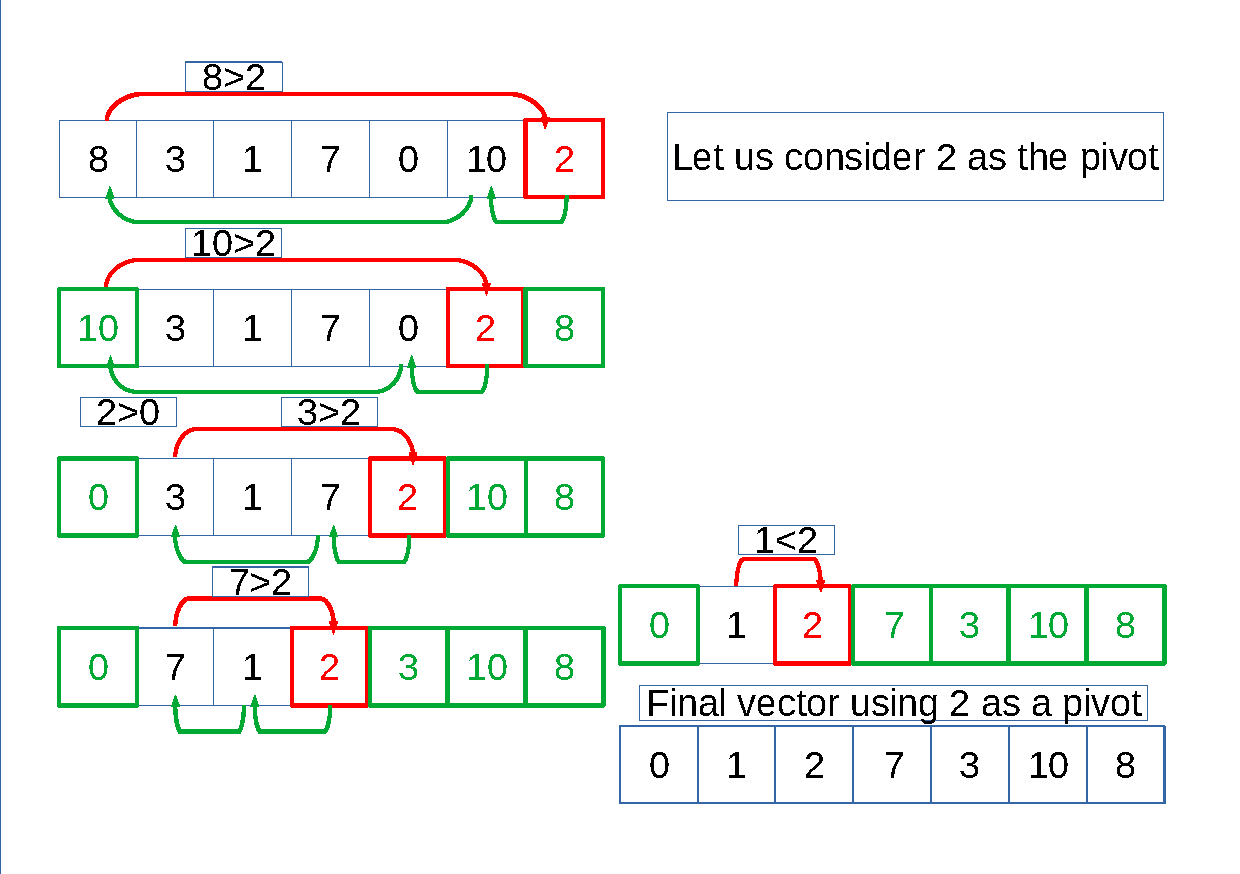
\includegraphics[scale=.6]{chapters/searchandsorting/images/sorting_8.pdf}
		\caption[Quicksort algorithm part one.]{Quicksort algorithm part one.}
		\label{sorting_8}
	\end{center}
\end{figure}

\begin{figure}[H]
	\begin{center}
		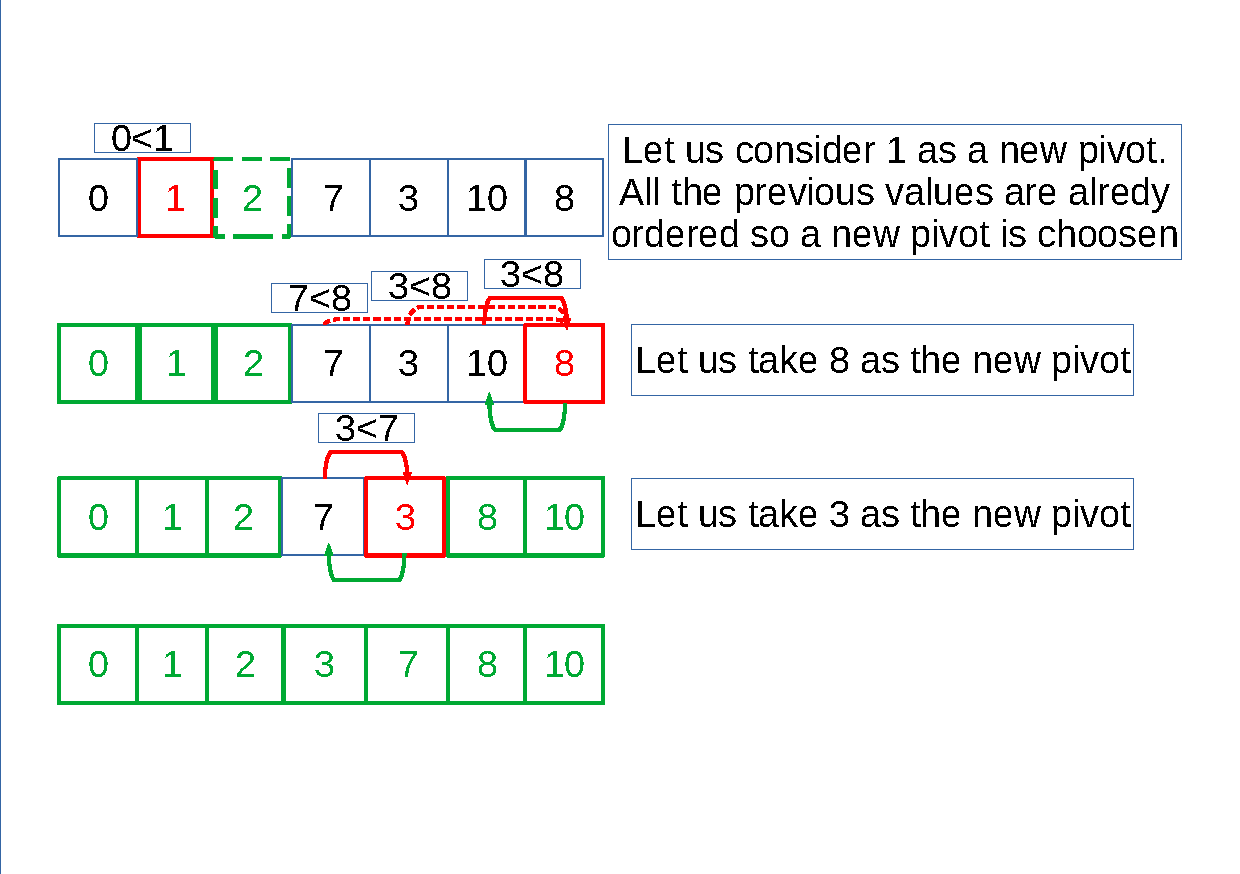
\includegraphics[scale=.6]{chapters/searchandsorting/images/sorting_9.pdf}
		\caption[Quicksort algorithm steps part two.]{Quicksort algorithm steps part two.}
		\label{sorting_9}
	\end{center}
\end{figure}

Here are the steps of quicksort algorithm based on the example of Figure \ref{sorting_8} and Figure \ref{sorting_9}:
\begin{itemize}
\item[1] Let us consider the last element as pivot, two in this case, and let us compare it with all the elements to its left. Let us start from the first element of the array, and let us compare their values. In this case \(8 > 2\), so \(8\) is moved on the position of the pivot (\(2\)) which is moved of one position to the left. The number to be removed, \(10\) in this case, is moved in the first position.
\item[2] Let us repeat the process. Now we have to compare the pivot (\(2\)) in the new position with the first element (\(10\)), and because \(10>2\) we repeat the previous step of moving the elements.
\item[3] In this case \(0<2\) so we do not have to do anything, but going to the next element, \(3\) in this case.
\item[4] For the pivot \(2\) all the elements to the left are less than it, and all the element to the right are bigger than it. \(2\) is not moved anymore. We can change the pivot and repeat all the steps for the new pivots until all the elements have been a pivot.
\end{itemize}

\subsection{Efficiency of the Quicksort Algorithm}
Evaluating the efficiency of quicksort is very hard. In the following there are some justifications for the worst case, and for the best and average complexity.

Let us consider first the worst case. In this situation the last elements of the array are the bigger ones, so it is necessary to check all the previous elements, by doing \(n^{2}\) comparisons Figure \ref{sorting_10}.

\begin{figure}[H]
	\begin{center}
		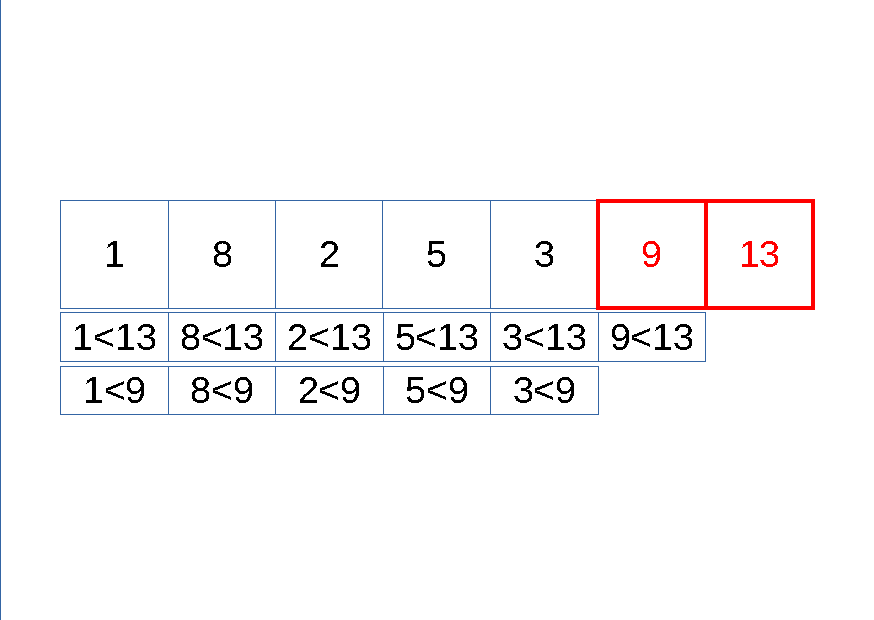
\includegraphics[scale=.6]{chapters/searchandsorting/images/sorting_10.pdf}
		\caption[Quicksort algorithm worst case.]{Quicksort algorithm worst case.}
		\label{sorting_10}
	\end{center}
\end{figure}

In the best and in the average case the complexity is \(O(n log(n)\). The reason is because the first pivot tends to move at the center of the array, having in this way two subarrays. The pivots of these two subarrays will tend to move at their center and the process is repeated until all the elements have been a pivot, having in this way an ordered array.

\begin{figure}[H]
	\begin{center}
		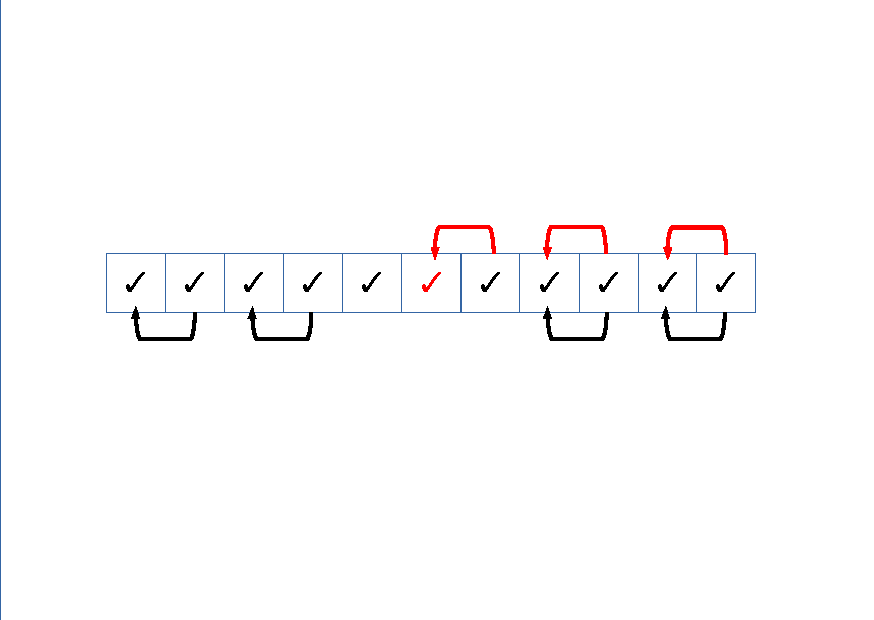
\includegraphics[scale=.6]{chapters/searchandsorting/images/sorting_11.pdf}
		\caption[Quicksort algorithm best and average case.]{Quicksort algorithm best and average case.}
		\label{sorting_11}
	\end{center}
\end{figure}

The space complexity of quicksort is constant, \(O(1)\).

This algorithm can be optimized in several ways. For example it is possible to order at the same time two half of the array, or considering as pivot always the last elements.

\paragraph{Quicksort and Merge Sort Comparison}
Quicksort is often a better solution than merge sort, because even if its worst case performance is \(O(n^{2})\), this problem can be solved by using the randomized quicksort. If the right pivot is chosen the problem related to having a worst case performance is solved. Moreover the quicksort algorithm dose not require an auxiliary memory, which is a big advance in a lot of situations.

On the other hand merge sort is a better solution than quicksort and heapsort \cite{wikiheapsort} (\href{https://en.wikipedia.org/wiki/Heapsort}{Heapsort, Wikipedia}) when the sorting is done on linked lists that do not require big auxilary space and on very large data sets stored on slow-to-access media, such as disk storage or network-attached storage \cite{wikiqicksort}.

\textbf{In summary}:
\begin{itemize}
\item \textbf{Worst Case}: \(O(n^{2})\)
\item \textbf{Average Case}: \(O(n\ log(n))\)
\item \textbf{Best Case}: \(O(n\ log(n))\)
\item \textbf{Space}: \(O(1)\)
\end{itemize}

\subsection{Quicksort Implementation}
The following code is the python implementation of the quicksort algorithm \cite{quicksortcode} (\href{https://www.educative.io/edpresso/how-to-implement-quicksort-in-python}{Quicksort Python Implementation}).
\begin{lstlisting}[firstnumber=1, caption={Quicksort python implementation.}]
def merge_sort(array_input):
	
	elements = len(array_input)
        
    # Base case
    if elements < 2:
    	return array_input
        
    # Position of the partitioning element
    current_position = 0

	# Partitioning loop
	for i in range(1, elements):
    	if array_input[i] <= array_input[0]:
        	current_position += 1
            temp = array_input[i]
            array_input[i] = array_input[current_position]
            array_input[current_position] = temp

    # Brings pivot to its appropriate position
    temp = array_input[0]
    array_input[0] = array_input[current_position]
    array_input[current_position] = temp
        
    # Sorts the elements to the left of pivot
    left = SortingAlgorithms.quicksort(array_input[0:current_position])
    # Sorts the elements to the right of pivot
    right = SortingAlgorithms.quicksort(array_input[current_position+1:elements])

    # Merging everything together
    array_input = left + [array_input[current_position]] + right

	return array_input
\end{lstlisting}

\begin{figure}[H]
	\begin{center}
		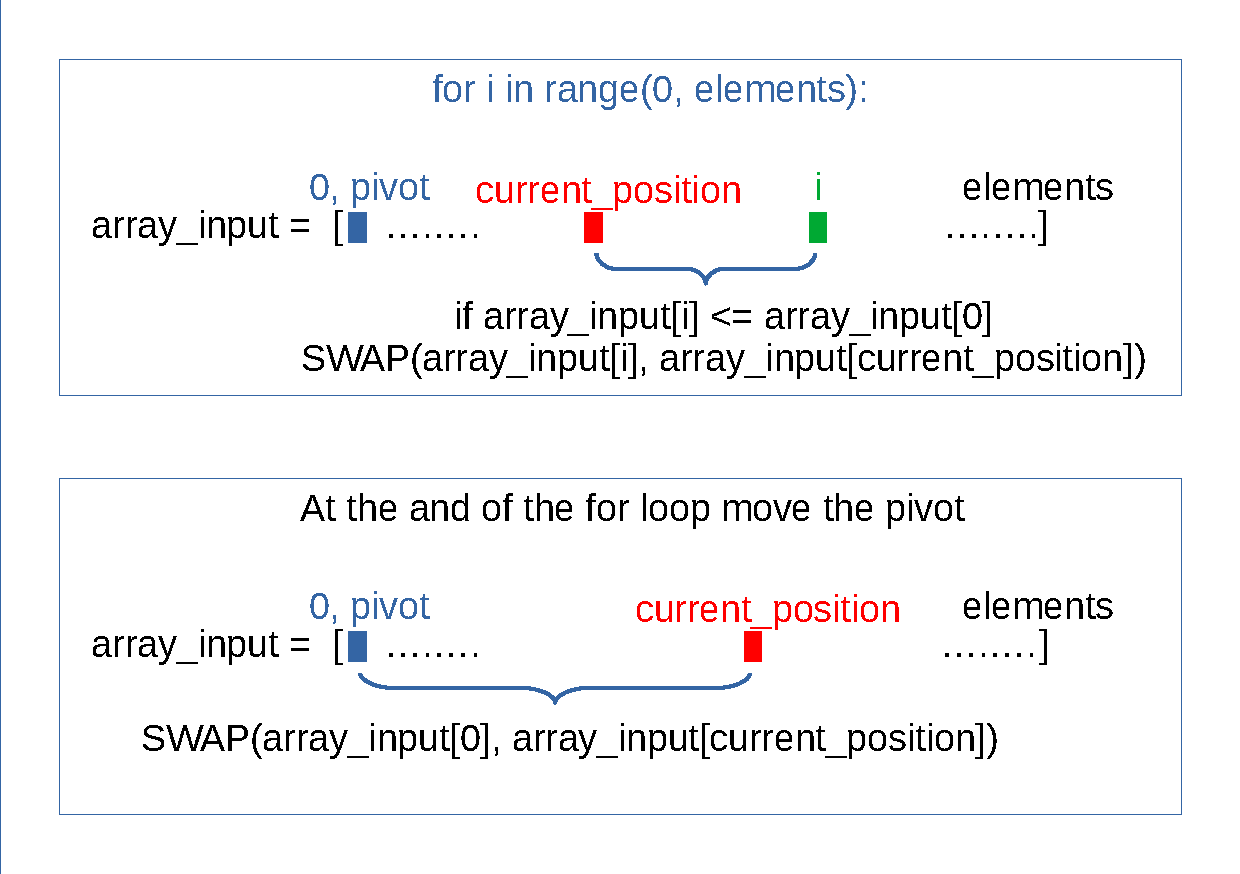
\includegraphics[scale=.6]{chapters/searchandsorting/images/sorting_12.pdf}
		\caption[Quicksort algorithm implementation.]{Quicksort algorithm implementation.}
		\label{sorting_12}
	\end{center}
\end{figure}
\chapter{Trees}
\label{chp: trees}
In this chapter are introduced the fundamentals concepts of tree as abstract data type, and the most used algorithms related to trees \cite{wikitrees} (\href{https://en.wikipedia.org/wiki/Tree_(data_structure)}{Trees, Wikipedia}).

\section{General Definitions}
A \textbf{tree} is an abstract datatype that simulate a hierarchical structure. A tree is a particular kind of a linked list where there are more next elements. The base element of a tree is called \textbf{node} while the first element is called \textbf{root}.

\begin{figure}[H]
	\begin{center}
		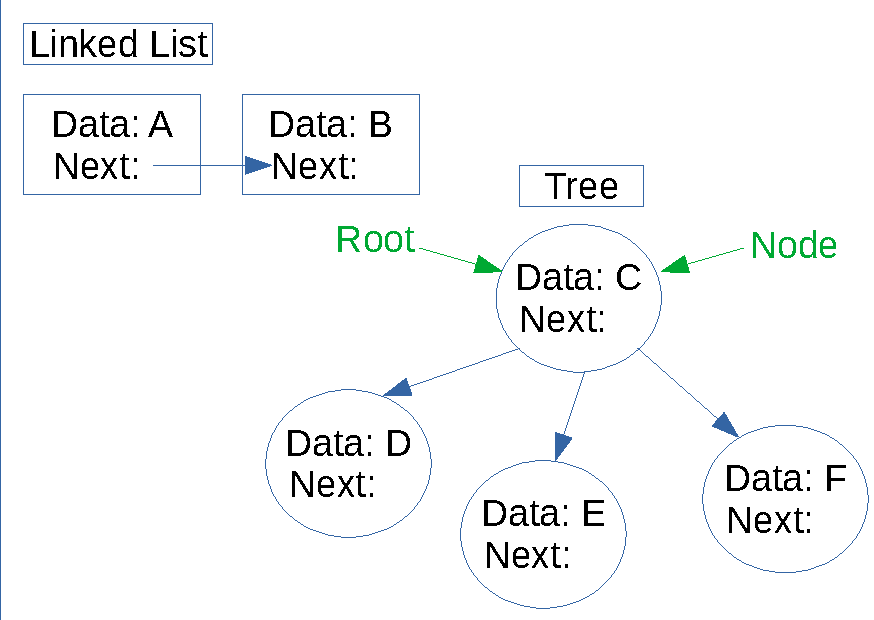
\includegraphics[scale=.6]{chapters/trees/images/trees_1.pdf}
		\caption[Elements of a tree and linked list.]{Elements of a tree and linked list.}
		\label{trees_1}
	\end{center}
\end{figure}

Trees must be completed connected structures, this means that there are not any nodes which are not connected to anything (Figure \ref{trees_2} case (a)), and there must not be present any cycles (Figure \ref{trees_2} case (c)).

\begin{figure}[H]
	\begin{center}
		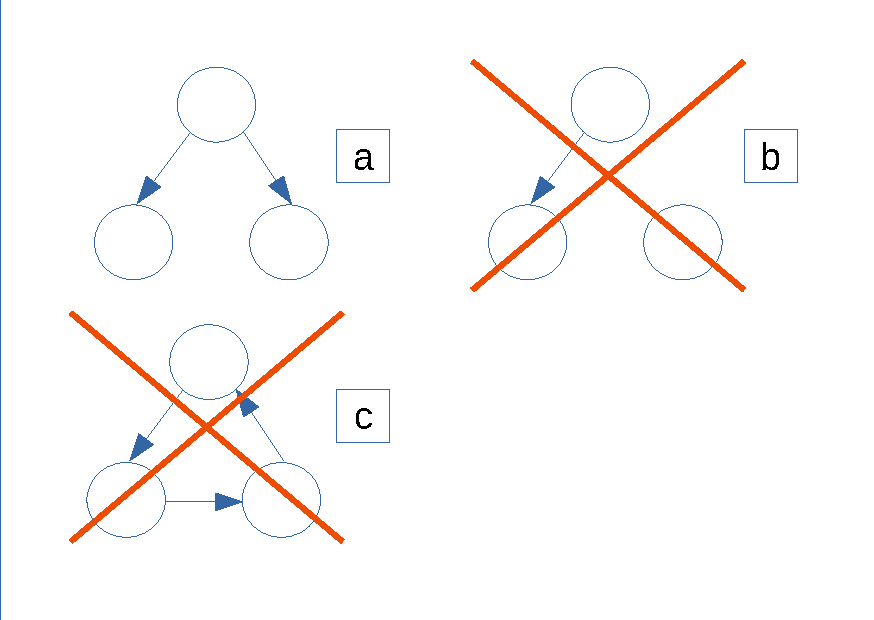
\includegraphics[scale=.6]{chapters/trees/images/trees_2.pdf}
		\caption[Possible structures of a tree.]{Completed connected structure (a), a non completed connected structure (b), and a cycle (c).}
		\label{trees_2}
	\end{center}
\end{figure}

Trees are a hierarchical structures divided into layers: the first layer is the one belonging to the root node, the first node of a tree. The next element of the root are called children, which became parents in case they have next node connected as well. The last nodes of a trees are the nodes which do not have any children and they are called \textbf{leaf}. The numbers of connections is called \textbf{height}. A set of connections creates a \textbf{path}. The numbers of edges starting from the root to a node is called \textbf{depth}.
All this definitions are defined in following figure (Figure \ref{trees_3}).

\begin{figure}[H]
	\begin{center}
		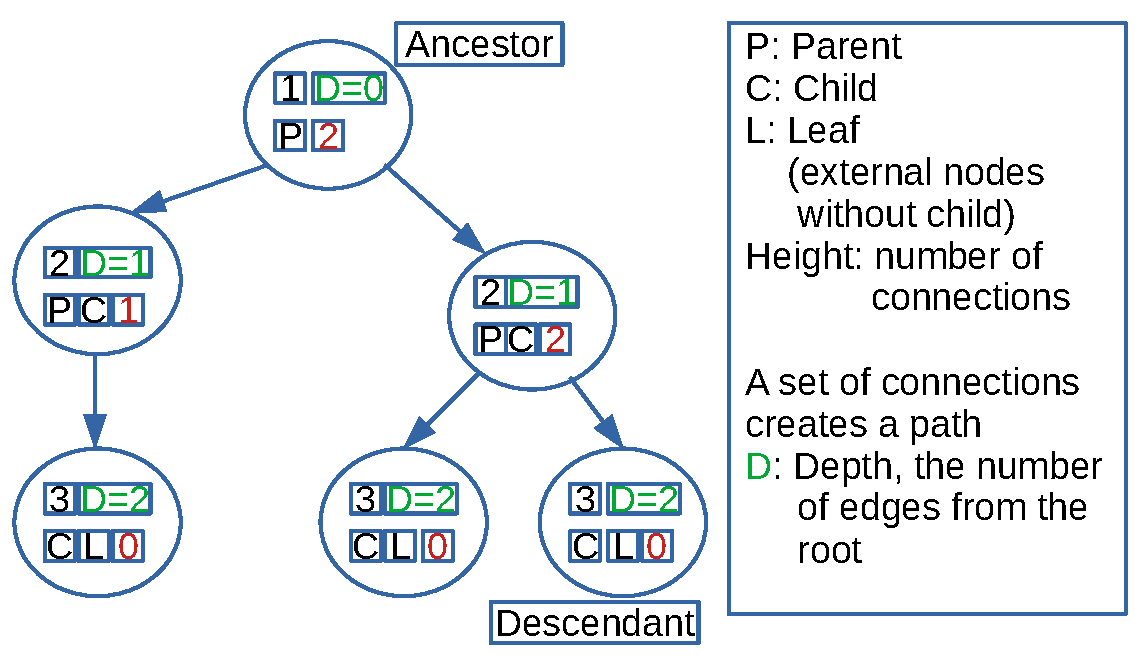
\includegraphics[scale=.6]{chapters/trees/images/trees_3.pdf}
		\caption[A tree and its fundamentals elements.]{A tree and its fundamentals elements.}
		\label{trees_3}
	\end{center}
\end{figure}

\section{Tree Traversal}
Which way is the most efficient for visiting all the nodes of a tree? Is it more efficient looking layer by layer or looking at subtrees? There are two different approach to traverse a tree: the \textbf{depth-first search} (\textbf{DFS}) and the \textbf{breath-first search} (\textbf{BFS}). In the first one the priority is to look at the children of a node, instead in the second one the priority is to look at the node of the same layer \ref{trees_4}.

\begin{figure}[H]
	\begin{center}
		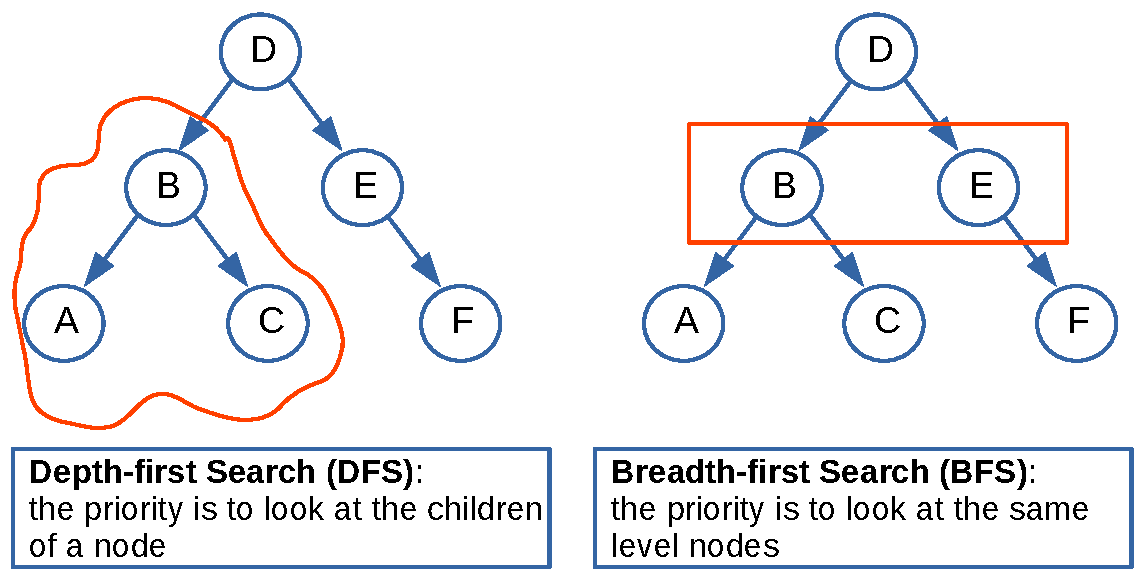
\includegraphics[scale=.6]{chapters/trees/images/trees_4.pdf}
		\caption[The depth-first search and the breath-first search.]{The depth-first search and the breath-first search.}
		\label{trees_4}
	\end{center}
\end{figure}

\subsection{Depth-first search}
In the depth-first search there are several different ways to perform a search on a tree.
\paragraph{Pre-order search}
\label{preorder}
In the \textbf{pre-order search} the first node to be checked as visited is the root. The following node is the left child by convention. Once checked the left child the process is repeated until the first node without any children is reached. At that point the same process is applied to the right side: all the nodes on the right are checked until all the nodes are checked as visited \ref{trees_5}.

\begin{figure}[H]
	\begin{center}
		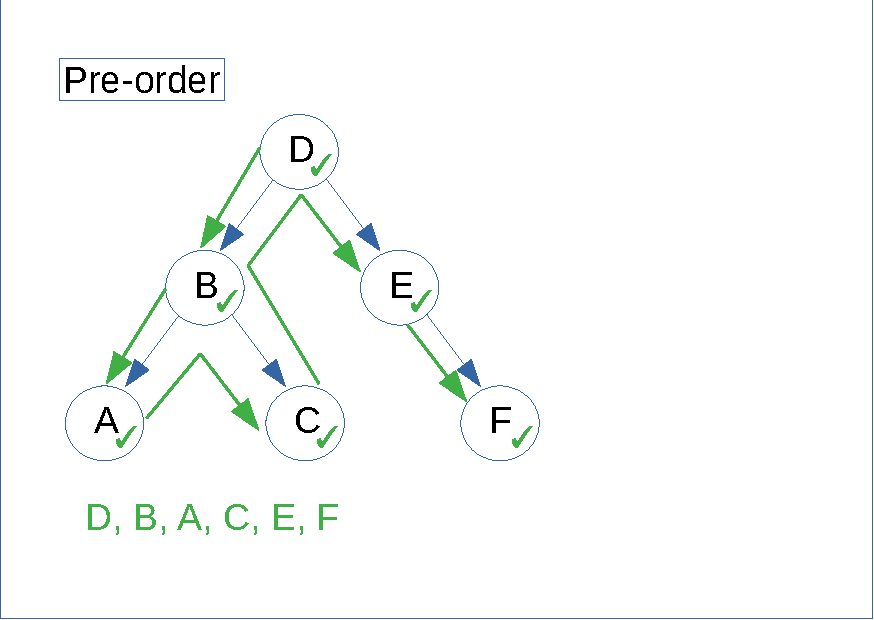
\includegraphics[scale=.6]{chapters/trees/images/trees_5.pdf}
		\caption[Pre-order search.]{Pre-order search.}
		\label{trees_5}
	\end{center}
\end{figure}

\paragraph{In-order search}
\label{inorder}
In the \textbf{in-order search} the first node to be checked is the first node without children on the left side. Once checked off this node the next one to be checked off is its parent, and the process is repeated again on the right side of the nodes, until all the nodes are checked off.

\begin{figure}[H]
	\begin{center}
		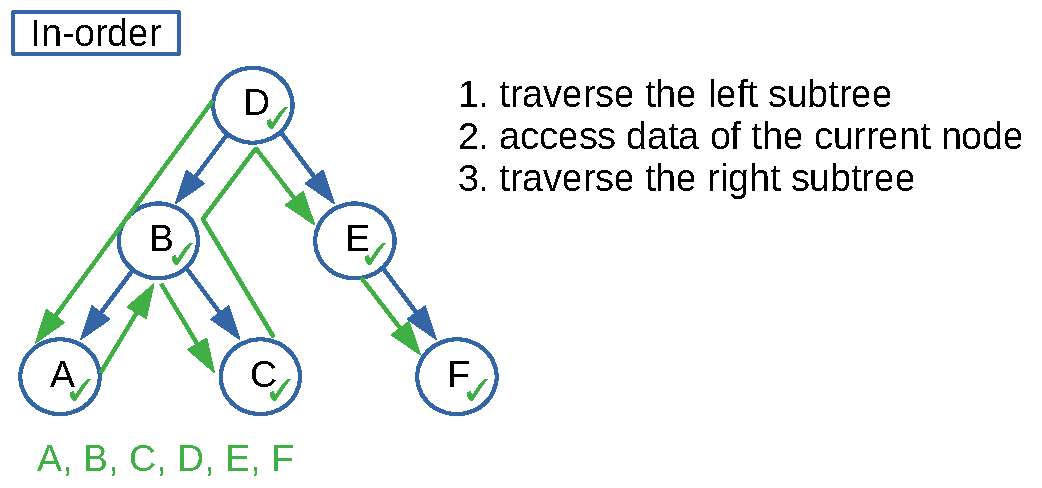
\includegraphics[scale=.6]{chapters/trees/images/trees_6.pdf}
		\caption[In-order search.]{In-order search.}
		\label{trees_6}
	\end{center}
\end{figure}

\paragraph{Post-order search}
\label{postorder}
In the \textbf{post-order search} the first node to be checked off is the first node without children on the left side. Once checked off this node the next one to be checked off is the one which does not have any children. Once all the nodes of the current left subtree without any children are checked off, the parents can be checked off, and the whole process is repeated until all the nodes are checked off.

\begin{figure}[H]
	\begin{center}
		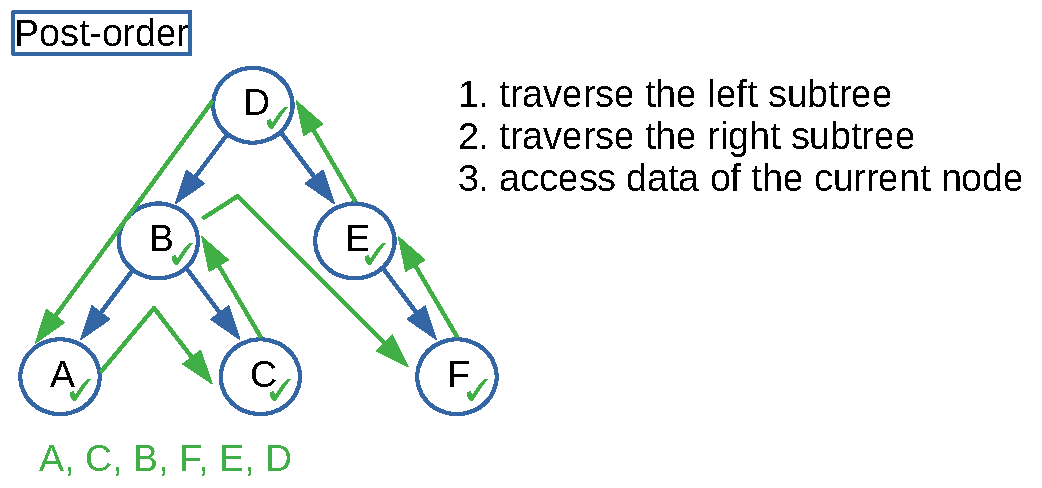
\includegraphics[scale=.6]{chapters/trees/images/trees_7.pdf}
		\caption[Post-order search.]{Post-order search.}
		\label{trees_7}
	\end{center}
\end{figure}

\section{Binary Trees}
\textbf{Binary trees} are trees in which the parent has at most two children (0, 1, 2 are the only number of admitted children). On binary trees some operations like searching, deleting, and inserting can be easily and efficiently done. 
\subsection{Search}
To search an element in the tree one of the previous methods can be used. Because in a general tree there is no ordering this means that potentially all the elements of the tree can be visited, then the complexity results in \(O(n)\).

\begin{figure}[H]
	\begin{center}
		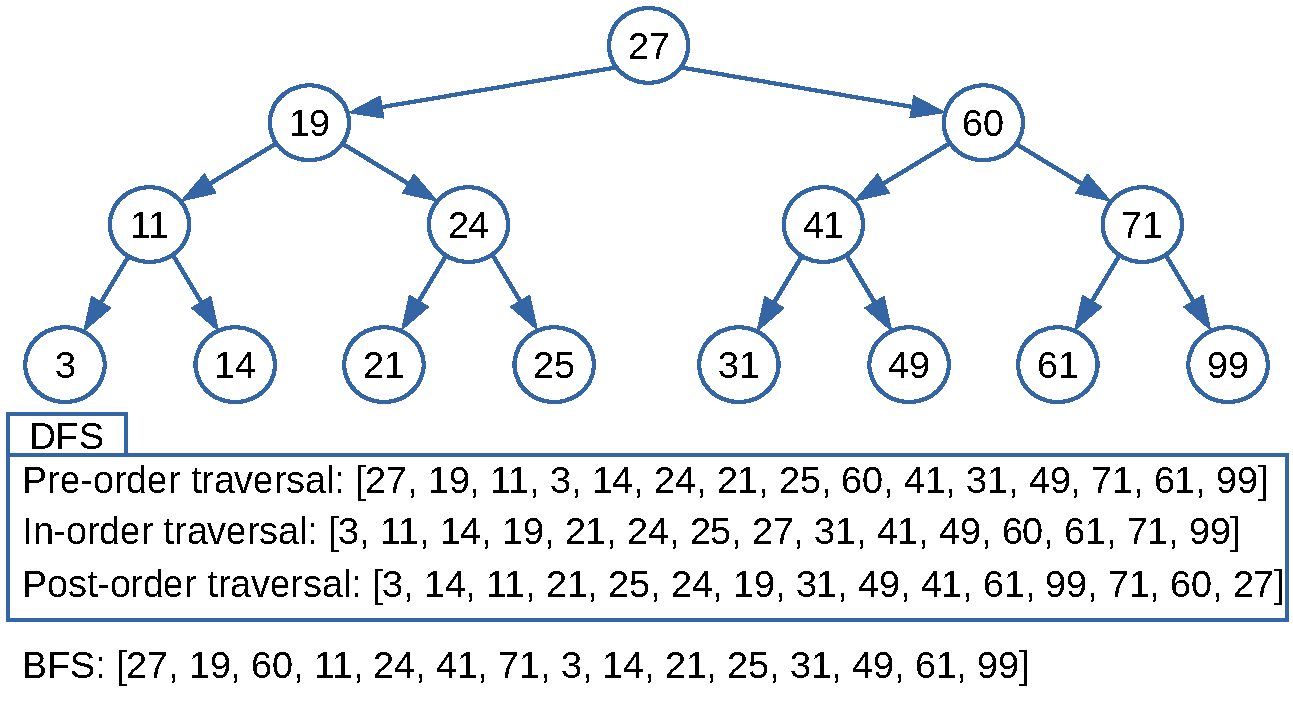
\includegraphics[scale=.6]{chapters/trees/images/trees_12.pdf}
		\caption[Example of tree search and traversal.]{Example of tree search and traversal.}
		\label{trees_12}
	\end{center}
\end{figure}

\subsection{Delete}
Before the delete process there is always a search one for finding the element to be deleted. If the element to be deleted is a leaf, deleting it is not a problem because there are not any children to be moved. Instead if the node to be removed has some children there are several opportunities to reorganize the nodes, because the condition for a binary tree must remain valid (a node can have at most two nodes). So there are several strategies. Let us consider the following tree \ref{trees_9}. 
\begin{itemize}
\item If the node to be removed has only one child it can be replaced by the child node (case 1 Figure \ref{trees_9}).
\item If the node to be removed has two children it can be replaced with the child node which has no children node (case 2 Figure \ref{trees_9}).
\item If the node to be removed has two children which have again children as well, in this case there are several options which can be done. For example on child node can be moved to the position of the one to be removed (case 3 Figure \ref{trees_9}).
\end{itemize} 

\begin{figure}[H]
	\begin{center}
		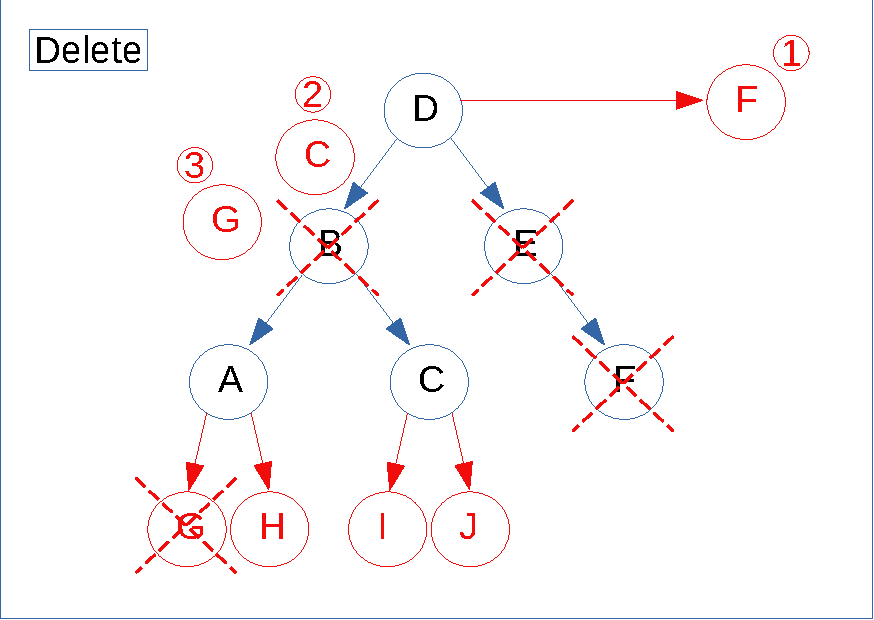
\includegraphics[scale=.6]{chapters/trees/images/trees_9.pdf}
		\caption[Delete an element of a tree.]{Delete an element of a tree.}
		\label{trees_9}
	\end{center}
\end{figure}
AGGIUNGERE IL LIBRO DI ALGORITMI CITANDO CHE SIA UNA LETTURA APPROFONDITA PER MAGGIORI DETTAGLI.
\subsection{Insert}
Insert a new element to a binary tree is not a hard operation, because it is enough to find a node which can take a new children node. In the worst case to find the proper node in which a child can be add the farthest leaf must be reached (case 1 \ref{trees_10}).

\begin{figure}[H]
	\begin{center}
		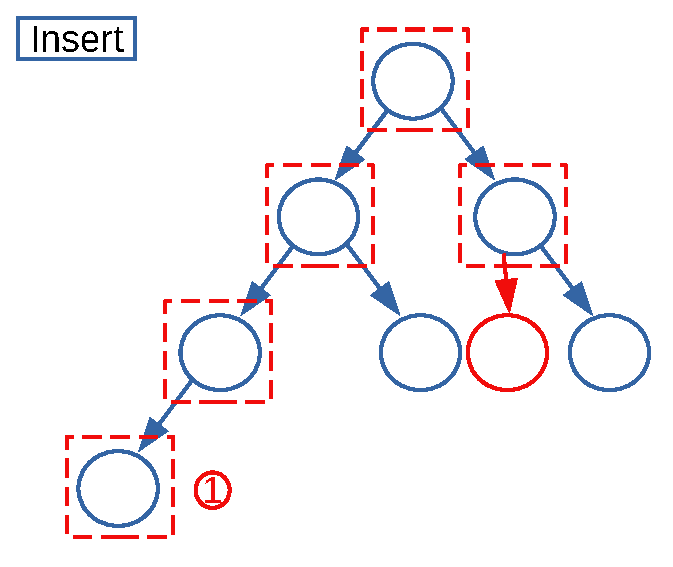
\includegraphics[scale=.6]{chapters/trees/images/trees_10.pdf}
		\caption[Add an element of a tree.]{Add an element of a tree.}
		\label{trees_10}
	\end{center}
\end{figure}
AGGIUNGERE IL LIBRO DI ALGORITMI CITANDO CHE SIA UNA LETTURA APPROFONDITA PER MAGGIORI DETTAGLI.
\subsection{Perfect binary tree}
A perfect binary tree is a binary tree in which all the nodes have two children except the leaf which do not have any children. In this case the following results are valid

\begin{figure}[H]
	\begin{center}
		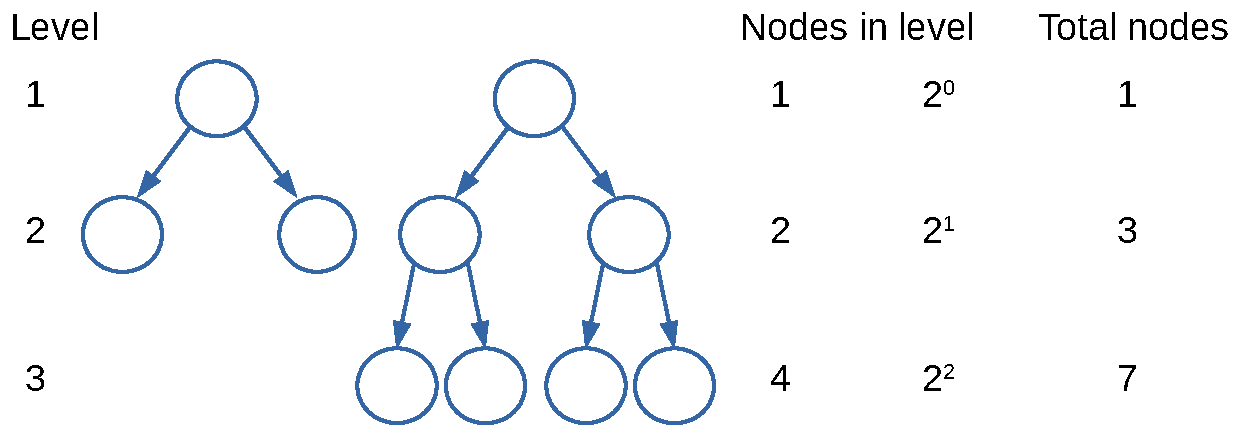
\includegraphics[scale=.6]{chapters/trees/images/trees_11.pdf}
		\caption[Perfect binary tree results.]{Perfect binary tree results.}
		\label{trees_11}
	\end{center}
\end{figure}

When a new row is added, the number of nodes double. Given a level \(n\) the total number of nodes is \(2n + 1\).

\subsection{Binary Tree Implementation}
The following code is the recursive Python implementation of the pre-order search and traversal (Figure \ref{trees_5}). The recursive and iterative implementations of the other ways of search and traverse a tree are in appendix \ref{binappendix}.

\begin{lstlisting}[firstnumber=1, caption={Class definition for a node and a tree.}]
class Node():

	def __int__(self, value):
		self.value = value
		self.left = None
		self.right = None

class BinaryTree():

	def __init__(self, root):
		self.root = Node(root)
\end{lstlisting}

\begin{lstlisting}[firstnumber=1, caption={Recursive pre-order traversal and search implementation.}]
class Node():
	...

class BinaryTree():
	...

	def print_tree(self):
		return self.preorder_print(tree.root, "")[:-1]

	def preorder_search_recursive(self, start, find_val):
		if start:
			if start.value == find_val:
				return True
			self.preorder_search_recursive(start.left, find_val)
			self.preorder_search_recursive(start.right, find_val)	
	
	def preorder_print(self, start, traversal):
		if start:
			traversal += (str(start.value) + "-")
			traversal = self.preorder_print(start.left, traversal)
			traversal = self.preorder_print(start.right,traversal)
		return traversal
\end{lstlisting}

\section{Binary Search Trees (BST)}
Performing operations such as search, addition, or removal of an element it is a very efficient process if the binary tree is ordered. A binary tree is ordered if for all nodes the left child has a minor value, and the right child has a greater value than the considered node \cite{wikibinsearchtree}(\href{https://en.wikipedia.org/wiki/Binary_search_tree}{Binary search tree, Wikipedia}).

\begin{figure}[H]
	\begin{center}
		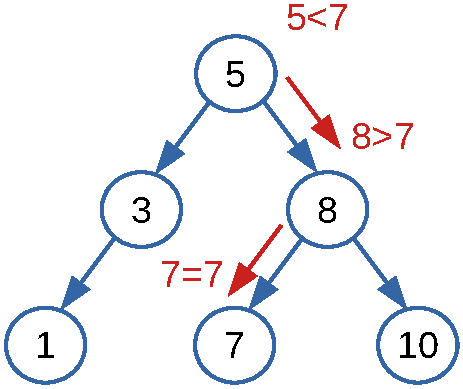
\includegraphics[scale=.6]{chapters/trees/images/trees_13.pdf}
		\caption[Search on an ordered binary tree.]{Search on an ordered binary tree.}
		\label{trees_13}
	\end{center}
\end{figure}

For example in Figure \ref{trees_13} is an ordered tree. Let us consider we would like to find the node which value is 7. Because the tree is ordered for efficiently finding 7 is enough to compare 7 with the value of the node and choose every time if to search on the right or on the left. In this way for finding a value is not mandatory to look at all the nodes, and the complexity for this operation is \(log(n)\).

Let us consider instead we would like to add a new node of value 4 to the tree of Figure \ref{trees_13}. Because the tree is ordered, there is only one place in which the node can be added. In the case of the tree in Figure \ref{trees_13} the node can be easily added because there is an empty space that can correctly take it (Figure \ref{trees_14}). In this case the complexity for this operation is again \(log(n)\).

\begin{figure}[H]
	\begin{center}
		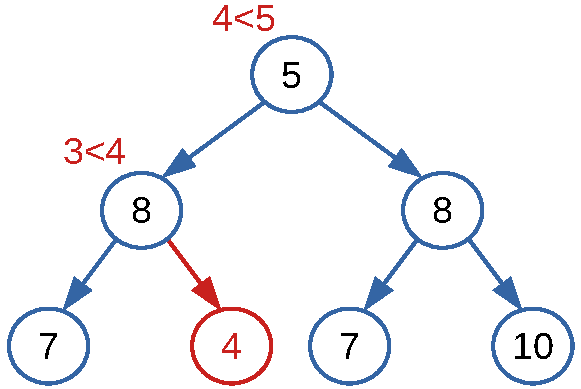
\includegraphics[scale=.6]{chapters/trees/images/trees_14.pdf}
		\caption[Addition on an ordered binary tree.]{Addition on an ordered binary tree.}
		\label{trees_14}
	\end{center}
\end{figure}

In case the position of the node is already occupied, adding the node could be a very difficult task. For a more complete and formal description of this topic refer to \cite{goodrich2013data} in the chapter about trees.

When all the possible nodes are present in each level the tree is said \textbf{balanced}. In Figure \ref{trees_14} there is an example of a balanced tree.
When instead a tree has all its children nodes which have always a bigger value, all the tree is on the right, and it is said to be \textbf{unbalanced}. In this case the search of an element has a \(O(n)\) complexity in the worst case.

\begin{figure}[H]
	\begin{center}
		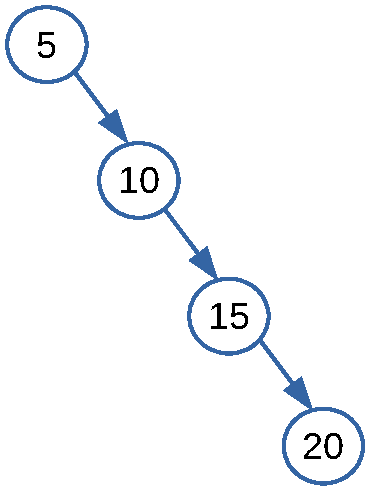
\includegraphics[scale=.6]{chapters/trees/images/trees_15.pdf}
		\caption[An unbalanced binary tree.]{An unbalanced binary tree.}
		\label{trees_15}
	\end{center}
\end{figure}

\subsection{Binary Search Tree Implementation}
The following code is the python implementation of the search and addition operations performed on a ordered binary tree.

\begin{lstlisting}[firstnumber=1, caption={implementation of insert and search operation for a binary search tree.}]
class BST():

	def __int__(self, root):
		self.root = Node(root)

	def insert(self, new_val):
		self.insert_helper(self.root, new_val)
	
	def insert_helper(self, current, new_val):
		if current.value < new_val:
			if current.right:
				self.insert_helper(current.right, new_val)
			else:
				self.current.right = Node(new_val)
		else:
			if current.left:
				self.insert_helper(current.left, new_val)
			else:
				current.left = Node(new_val)
	
	def search(self, find_val):
		return self.search_helper(self.root, find_val)
	
	def search_helper(self, current, find_val):
		if current:
			if current.value == find_val:
				return True
			elif current.value < find_val:
				return self.search_helper(current.right, find_val)
			else:
				return self.search_helper(current.left, find_val)
		return False
\end{lstlisting}

\section{Heaps}
\textbf{Heaps} are particular tree-based data structure in which the elements are ordered in increasing or decreasing order \cite{wikiheap} (\href{https://en.wikipedia.org/wiki/Heap_(data_structure)}{Heap, Wikipedia}). Heaps are a very efficient implementation of the abstract data type (Chapter \ref{chp:datastrucutres}) priority queue (Section \ref{queue}). The value with the highest (or lowest) priority is always stored at the root. Heaps are very useful when an element with a high (or low) priority must be repeatedly removed from the heap. Moreover, heaps are not sorted structure, but are regarded as partially ordered.    

We say the \textit{max heap} (Figure \ref{trees_16} (a)) if for every node its children have the values less or equal than the one of the parent (the root has always the highest value). We say instead \textit{min heap} (Figure \ref{trees_16} (b)) if for every node its children have the values higher or equal than the on of the parent (the root has the lowest value).

\begin{figure}[H]
	\begin{center}
		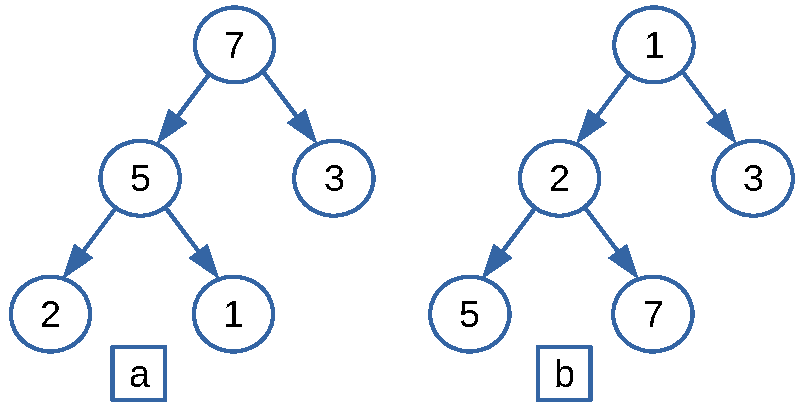
\includegraphics[scale=.6]{chapters/trees/images/trees_16.pdf}
		\caption[Max heap and min heap example.]{Max heap and min heap example.}
		\label{trees_16}
	\end{center}
\end{figure}

In general heaps are not binary trees so they can have more than two nodes.

In a max heap tree the search of the biggest value is called \textbf{peek} and it has a constant complexity (\(O(1)\)). For searching other values instead we have to check node by node as the ordering of the left and right side is not guarantee. The average case is \(O(\frac{n}{2})\ = \ O(n)\).
\subsection{Heapify}
Let us consider we would like to add a new node to a heap. In this case the node to be add must respect the heap condition. For doing so the node is added in the first available position, and later the node of the heap are swapped in order to keep true the heap condition.

\begin{figure}[H]
	\begin{center}
		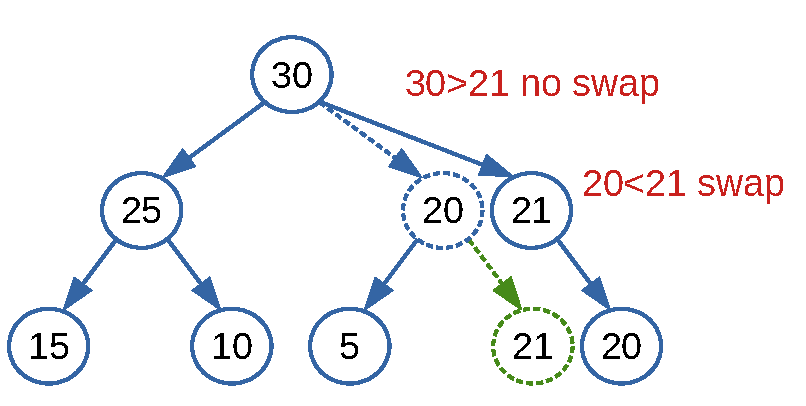
\includegraphics[scale=.6]{chapters/trees/images/trees_17.pdf}
		\caption[Add a new node to a heap.]{Add a new node to a heap.}
		\label{trees_17}
	\end{center}
\end{figure}

In the example of Figure \ref{trees_17} only one swap is necessary. The complexity of adding a new element and swap all the node, in order to keep valid the heap condition, is \(log(n)\), and in the worst case the highest number of operations correspond to the height of the tree.

\subsection{Heap Implementation}
To implement a heap we can use an array. An example of this application is shown in the following figure (Figure \ref{trees_18}).

\begin{figure}[H]
	\begin{center}
		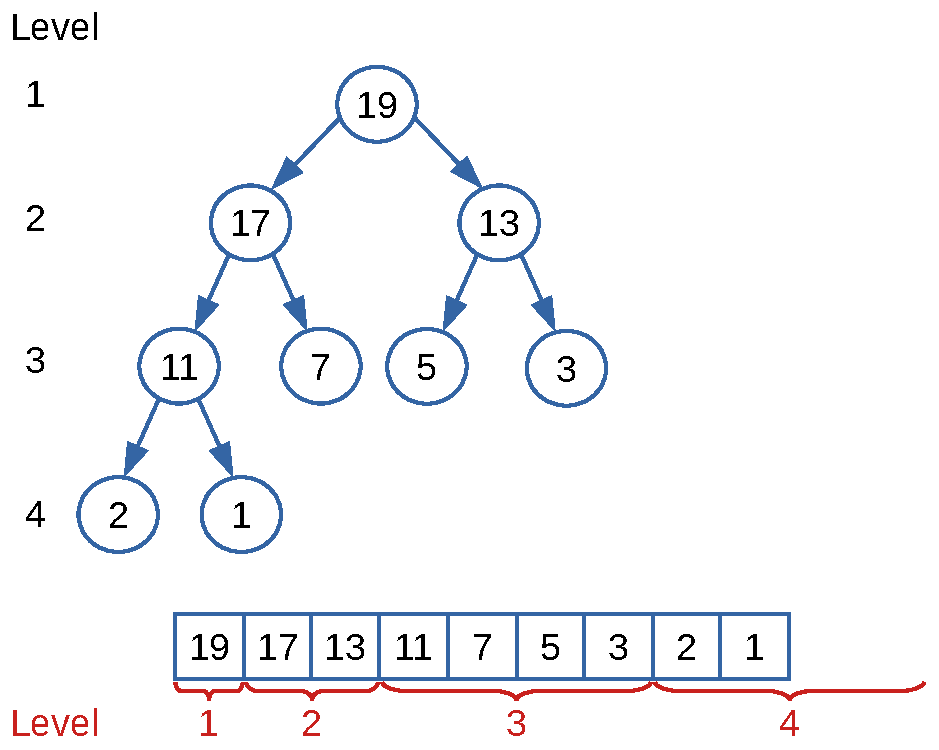
\includegraphics[scale=.6]{chapters/trees/images/trees_18.pdf}
		\caption[Implementation example of a heap using an array.]{Implementation example of a heap using an array.}
		\label{trees_18}
	\end{center}
\end{figure}

\section{Self-balancing Binary Search Trees}
\textbf{Self-balancing binary trees} are binary tree-based structure that automatically maintain the lowest height (number of levels below the root) when an insertion or deletion is done \cite{wikiselfbalancing} (\href{https://en.wikipedia.org/wiki/Self-balancing_binary_search_tree}{Self-balancing binary search tree, Wikipedia}). This structure is an efficient way to implement abstract data type like lists, priority queue, and sets.

\begin{figure}[H]
	\begin{center}
		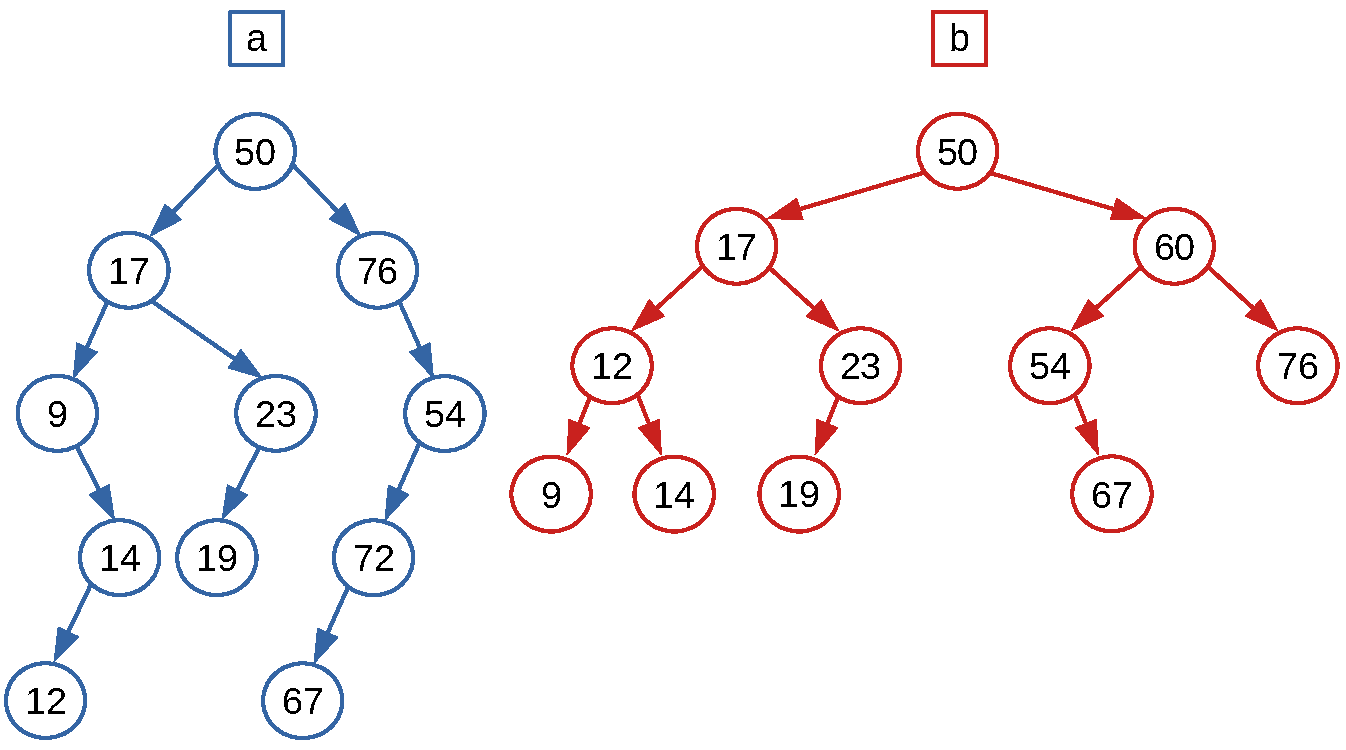
\includegraphics[scale=.6]{chapters/trees/images/trees_19.pdf}
		\caption[Example of balancing an unbalanced tree.]{Example of balancing an unbalanced tree. Credits: \href{https://en.wikipedia.org/wiki/Self-balancing_binary_search_tree}{Self-balancing binary search tree, Wikipedia}}
		\label{trees_19}
	\end{center}
\end{figure}

In Figure \ref{trees_19} is show an unbalanced tree (case a) in which the average path to reach the leaf is 3.27 nodes. If the same tree is balanced (case b) the average path to reach any leaf from the root decreased to 3.

\section{Red-Black Trees}
The \textbf{red-black trees} are particular kind of self balancing trees. An extra bit is used to store the color of the node, which can be only \textbf{red} or \textbf{black}. Using a color for each node assures that the tree remains balanced during insertion and deletion operations \cite{wikiblackred} (\href{https://en.wikipedia.org/wiki/Red%E2%80%93black_tree}{Red-black tree, Wikipedia}).

The rules that a red-black tree must respect are:
\begin{itemize}
\item[1] Nodes can be only of two types: \textbf{red} or \textbf{black}.
\item[2] There must exist the \textbf{null leaf nodes}. Every node which does not have two leaf must have the children \textbf{null}.
\item[3] If a node is \textbf{red} all its children must be \textbf{black}.
\item[4] Usually the root is \textbf{black}, but this is not mandatory.
\item[5] Every path from a the upper nodes to the lower ones must contain the same number of \textbf{black} nodes. This property is very important when inserting new nodes.
\end{itemize}

\begin{figure}[H]
	\begin{center}
		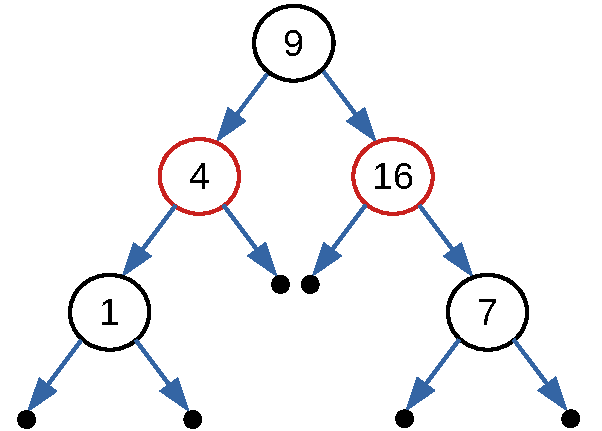
\includegraphics[scale=.6]{chapters/trees/images/trees_20.pdf}
		\caption[A red-black tree.]{A red-black tree.}
		\label{trees_20}
	\end{center}
\end{figure}

Usual only red nodes are added and the color of the other nodes are changed accordingly in order to respect the rule for the red-black tree.

\begin{figure}[H]
	\begin{center}
		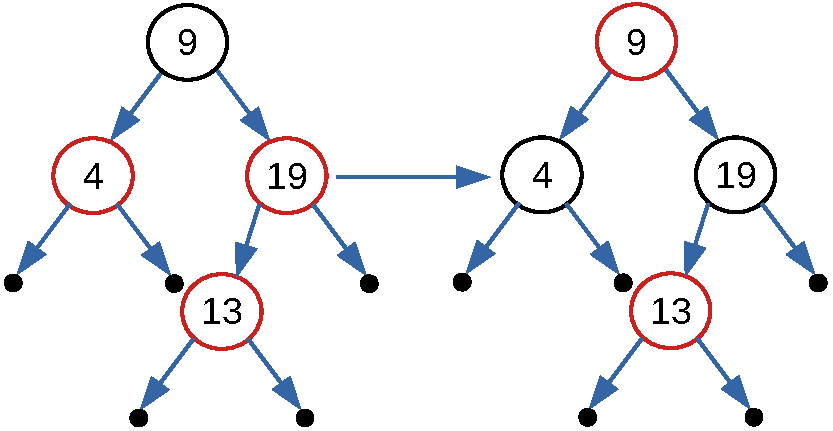
\includegraphics[scale=.6]{chapters/trees/images/trees_21.pdf}
		\caption[Insertion of a new node and the following updating of the color nodes.]{Insertion of a new node and the following updating of the color nodes.}
		\label{trees_21}
	\end{center}
\end{figure}

In case the insertion or the removal does nor respect the rules of the red-black tree and BST some more complex operations must be done as in the following figure.

\begin{figure}[H]
	\begin{center}
		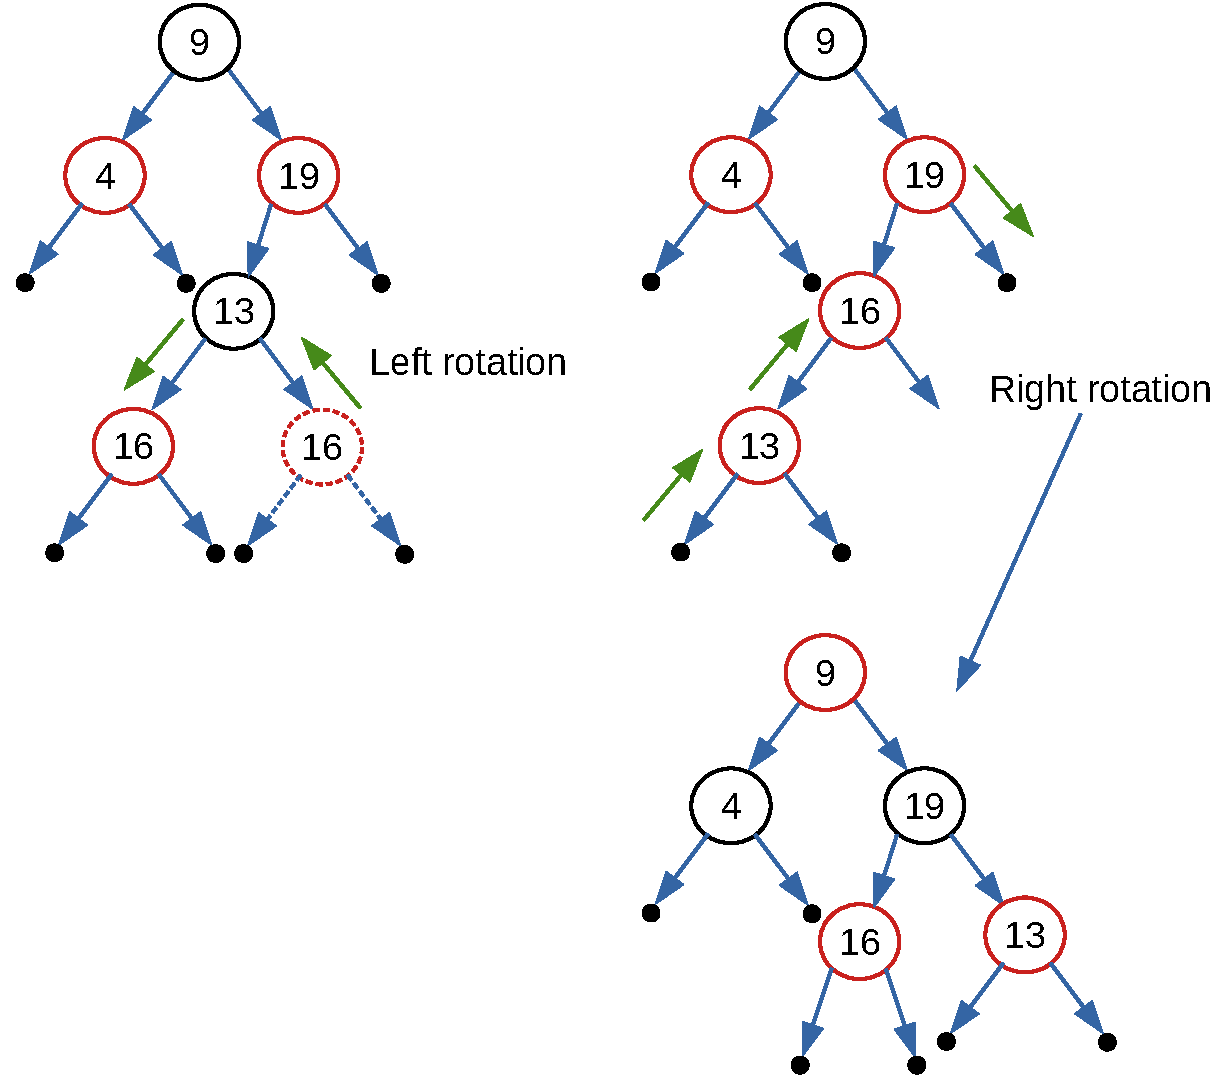
\includegraphics[scale=.6]{chapters/trees/images/trees_22.pdf}
		\caption[Left and right rotation for balancing the tree after an insertion.]{Left and right rotation for balancing the tree after an insertion.}
		\label{trees_22}
	\end{center}
\end{figure}
\clearpage

% Bibliography
\defbibnote{bibnote}{\par\bigskip}
\printbibliography[heading=bibintoc, title=Bibliography, prenote=bibnote]
\end{document}